\documentclass{ctexart}
\usepackage{amsmath}
\usepackage{float}
\usepackage{amssymb}
\usepackage{graphicx}
\usepackage{gbt7714}
\usepackage{pifont}
\usepackage{wrapfig}
\usepackage{multirow}
\usepackage{array}

\ctexset{
    % 修改 section。
    section={   
        name={,、},
        number={\chinese{section}}
    }
}

\title{磁滞回线}
\author{陆知辰-10225301478}
\date{\today}
\graphicspath{{figure/}}

\begin{document}

\begin{titlepage}
  \centering
  % 插入图片
  
\includegraphics[width=0.5\textwidth]{ecnu.png}
  
  % 空行用于调整标题位置
  \vspace*{\baselineskip}
  
  % 标题
  \Huge\textbf{物\quad 理\quad 实\quad 验 \quad (二)}
  % 空行用于调整标题和其他信息之间的间距
  \vspace*{0.3\baselineskip}
  
  % 具体实验名称
  \huge 磁滞回线
  
  % 空行用于调整时间和其他信息之间的间距
  \vspace*{2\baselineskip}
  
  % 时间
  \large 时间:\today
  
  % 空行用于调整时间和其他信息之间的间距
  \vspace*{\baselineskip}
  
  % 创作人
  \large 创作人:陆知辰
  
  % 空行用于调整创作人和学号之间的间距
  \vspace*{\baselineskip}
  
  % 学号
  \large 学号:10225301478
  
\end{titlepage}
\newpage
\tableofcontents
\newpage
\section{实验摘要}
  \subsection{实验概要}
  铁磁物质是一种性能特异、用途广泛的材料.铁、钴、镍及其众多合金以及含铁的氧化物均属铁磁物质,
  铁磁物质的一个特征是在外磁场作用下能被强烈磁化,故铁磁物质的磁导率很高,铁磁物质的另一个特征是磁滞现象,即磁化场停止作用后,
  铁磁物质仍会保留磁化状态,磁滞现象有着广泛的应用.

  \subsection{实验目的}
  1.\quad 认识铁磁物质的磁化规律,比较不同铁磁材料的动态磁化特性。

  2.\quad 了解利用示波器测量铁磁材料动态磁滞回线的原理和方法。
  
  3.\quad 测绘铁磁样品的磁滞回线和基本磁化曲线。

\section{实验原理}
  \subsection{铁磁材料的磁滞现象}
  图\ref{tieciqvxian}为铁磁物质磁感应强度B与磁场强度H之间的关系曲线。
  图中的原点O表示磁化之前铁磁物质处于磁中性状态,即B=0,H=0.当磁场的H从零开始增加时,磁感应强度B随之缓慢上升,
  如线段Oa所示;继之B随H迅速增长,如线段ab所示;其后B的增长又趋缓慢,并当H增至Hm时,
  B到达饱和值.OabS称为起始磁化曲线。
  当磁场从Hm逐渐减小至零,磁感应强度B并不沿起始磁化曲线恢复到原点O,
  而是沿另一条新曲线SR下降。
  比较线段OS和SR可知,减小B相应也减小,但B的变化滞后于H的变化,这种现象称为磁滞,磁滞的明显特征是当H=0时,B不为零,而保留剩磁B。

  \begin{figure}[H]\label{tieciqvxian}
    \centering
    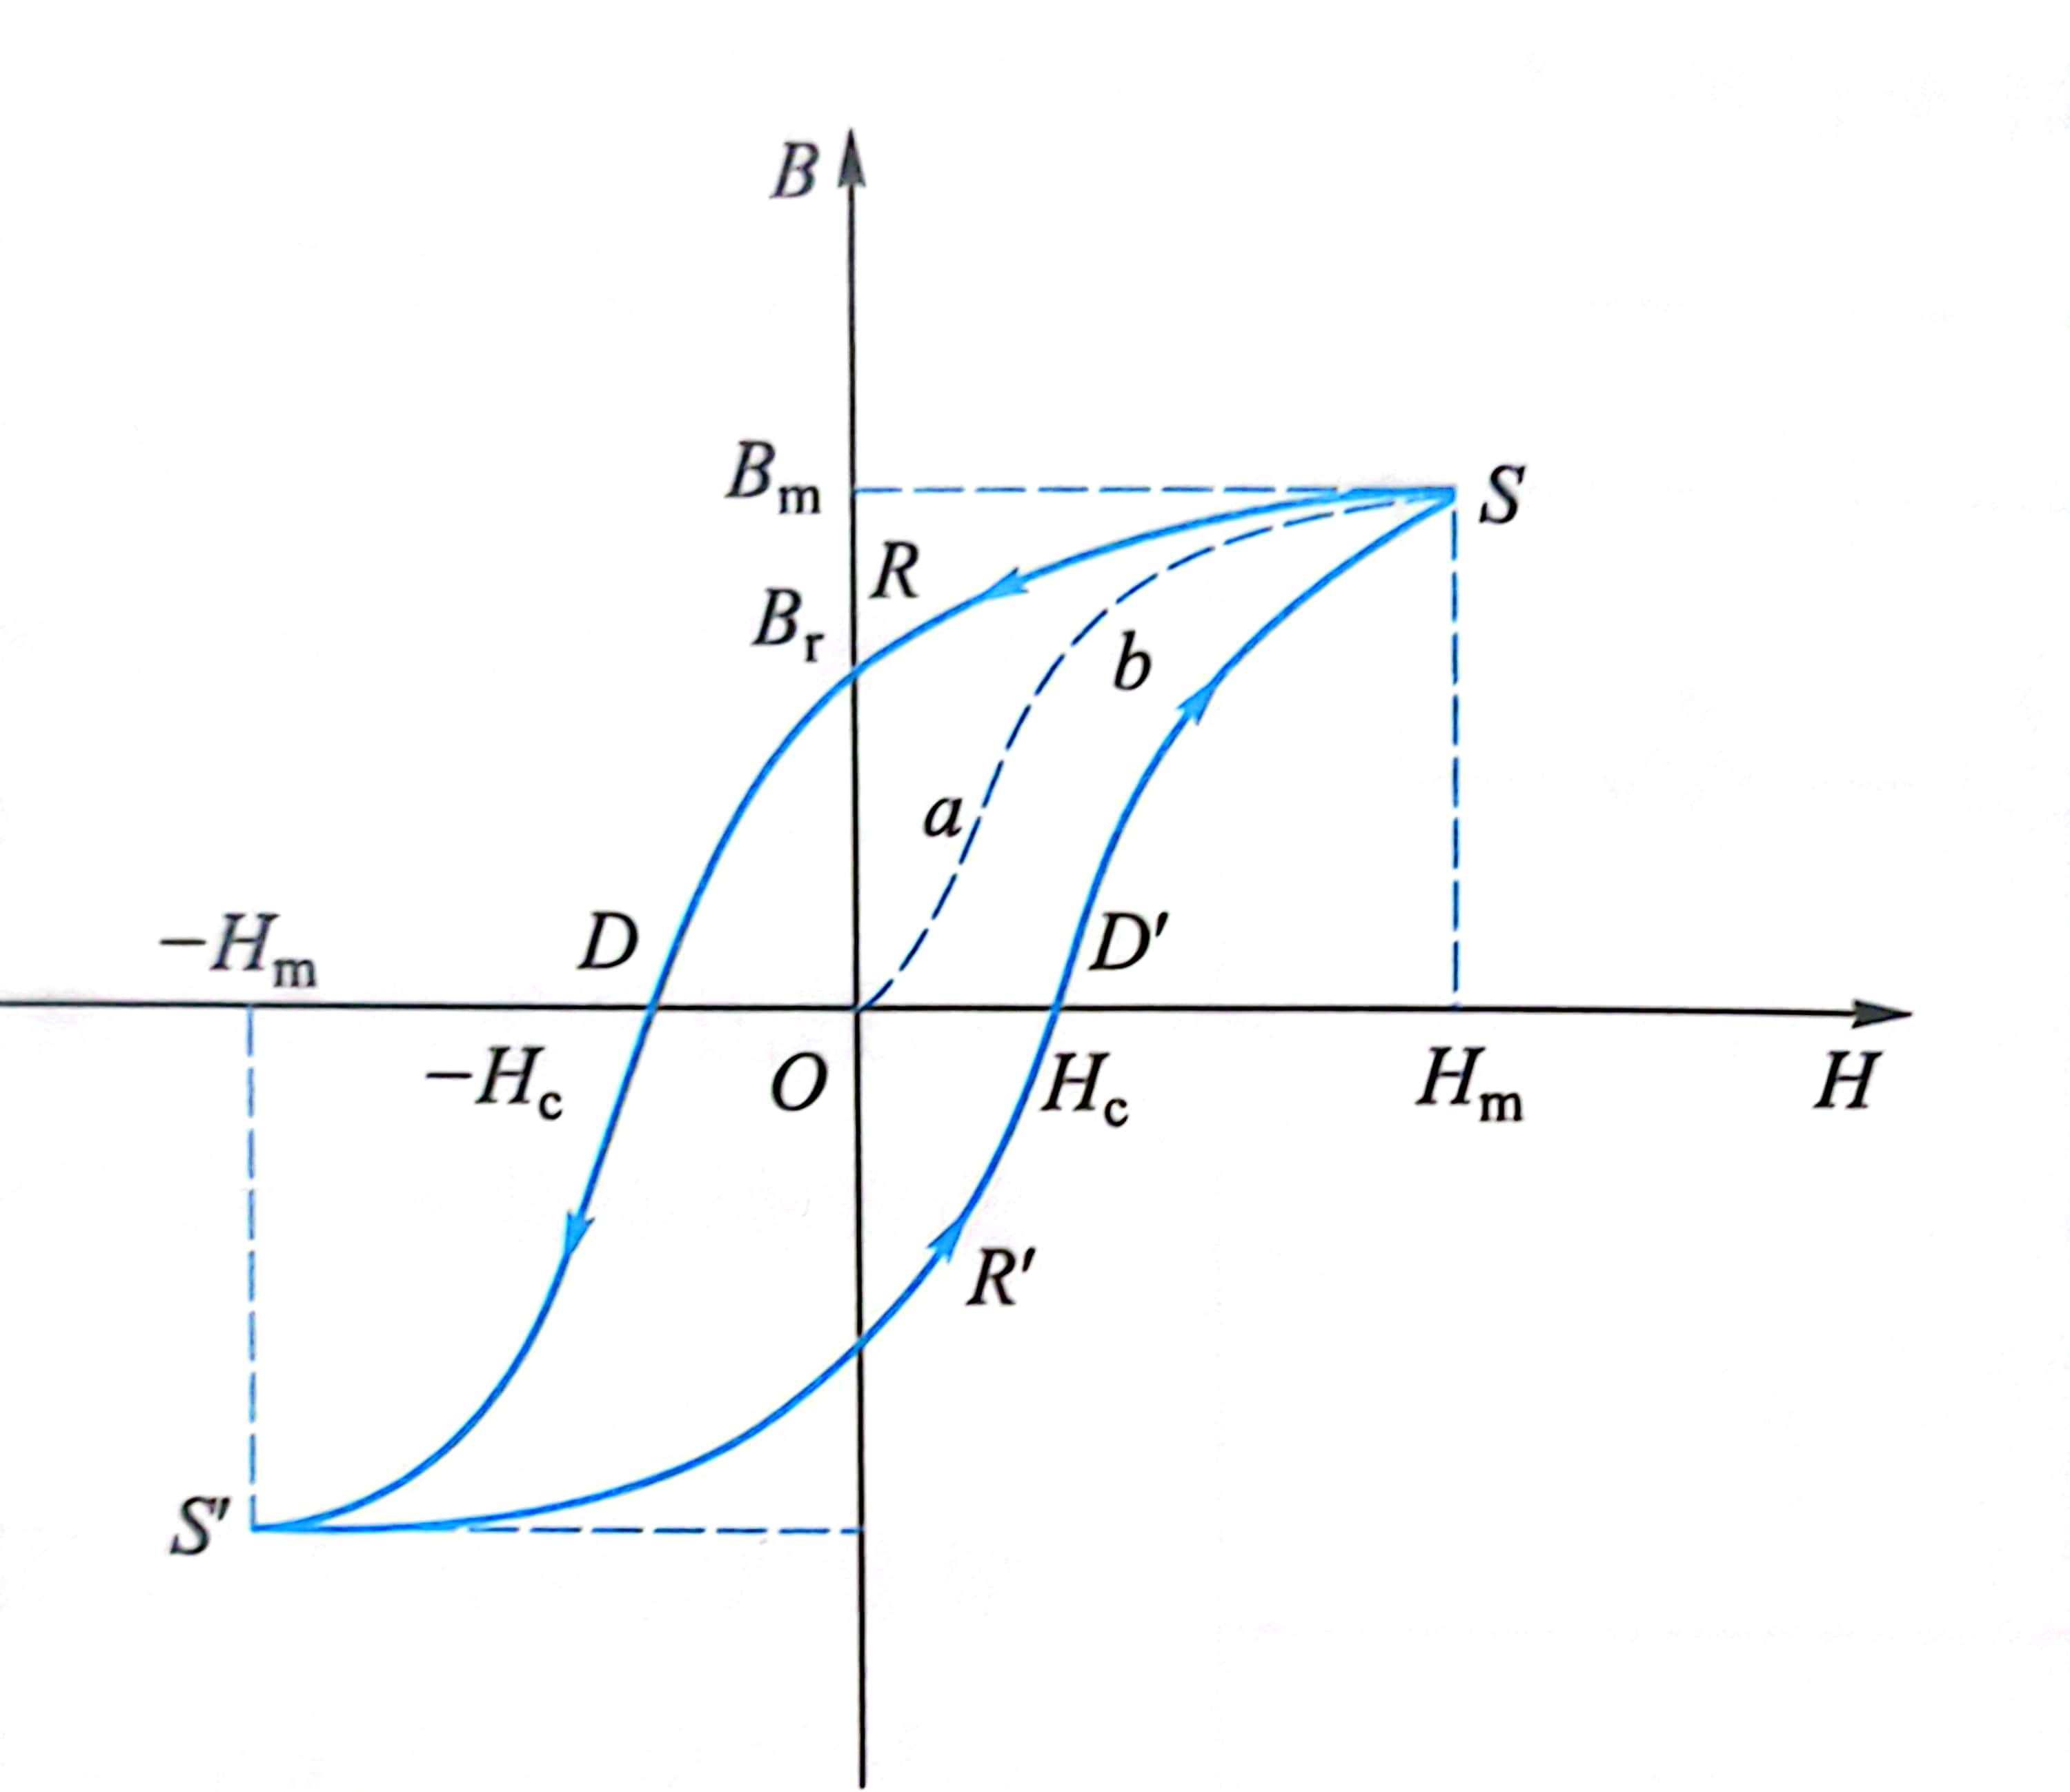
\includegraphics[width=0.8\textwidth,height=0.4\textheight]{tieciqvxian.jpg}
    \caption{铁磁材料磁滞回线}
  \end{figure}

  当磁场反向从O逐渐变至$-H_{e}$。时,磁感应强度B消失.这说明要消除剩磁,
  必须施加反向磁场,$H_{e}$称为矫顽力,它的大小反映铁磁材料保持剩磁状态的能力,线段RD称为退磁曲线。

  图\ref{tieciqvxian}还表明,当磁场按$$H_{m}\rightarrow 0\rightarrow -H_{e}\rightarrow -H_{m}\rightarrow 0\rightarrow H_{e}\rightarrow H_{m}$$
  次序变化,相应的磁感应强度B则沿闭合曲线SRDS'R'D'S'变化,这条闭合曲线称为磁滞回线。
  所以,当铁磁材料处于交变磁场中时(如变压器中的铁芯),将沿磁滞回线反复被磁化→去磁→反向磁化→反向去磁,
  在此过程中要消耗额外的能量,并以热的形式从铁磁材料中释放,这种损耗称为磁滞损耗,可以证明,磁滞损耗与磁滞回线所围面积成正比。

  应该说明,当初始态为H=0,B=0的铁磁材料,在交变磁场强度由弱到强依次进行磁化,可以得到面积由小到大向外扩张的一簇磁滞回线,
  如图\ref{tongyicailiaoqvxian}所示.这些磁滞回线顶点的连线称为铁磁材料的基本磁化曲线,由此可近似确定其磁导率$\mu =\frac{B}{H}$。
  因B与H的关系成非线性,故铁磁材料的$\mu$不是常数,
  而是随H而变化,如图\ref{muH}所示.铁磁材料的相对磁导率可高达数千乃至数万,这一特点是它用途广泛的主要原因之一。

  \begin{figure}[H]
    \begin{minipage}[t]{0.45\textwidth}
      \centering
      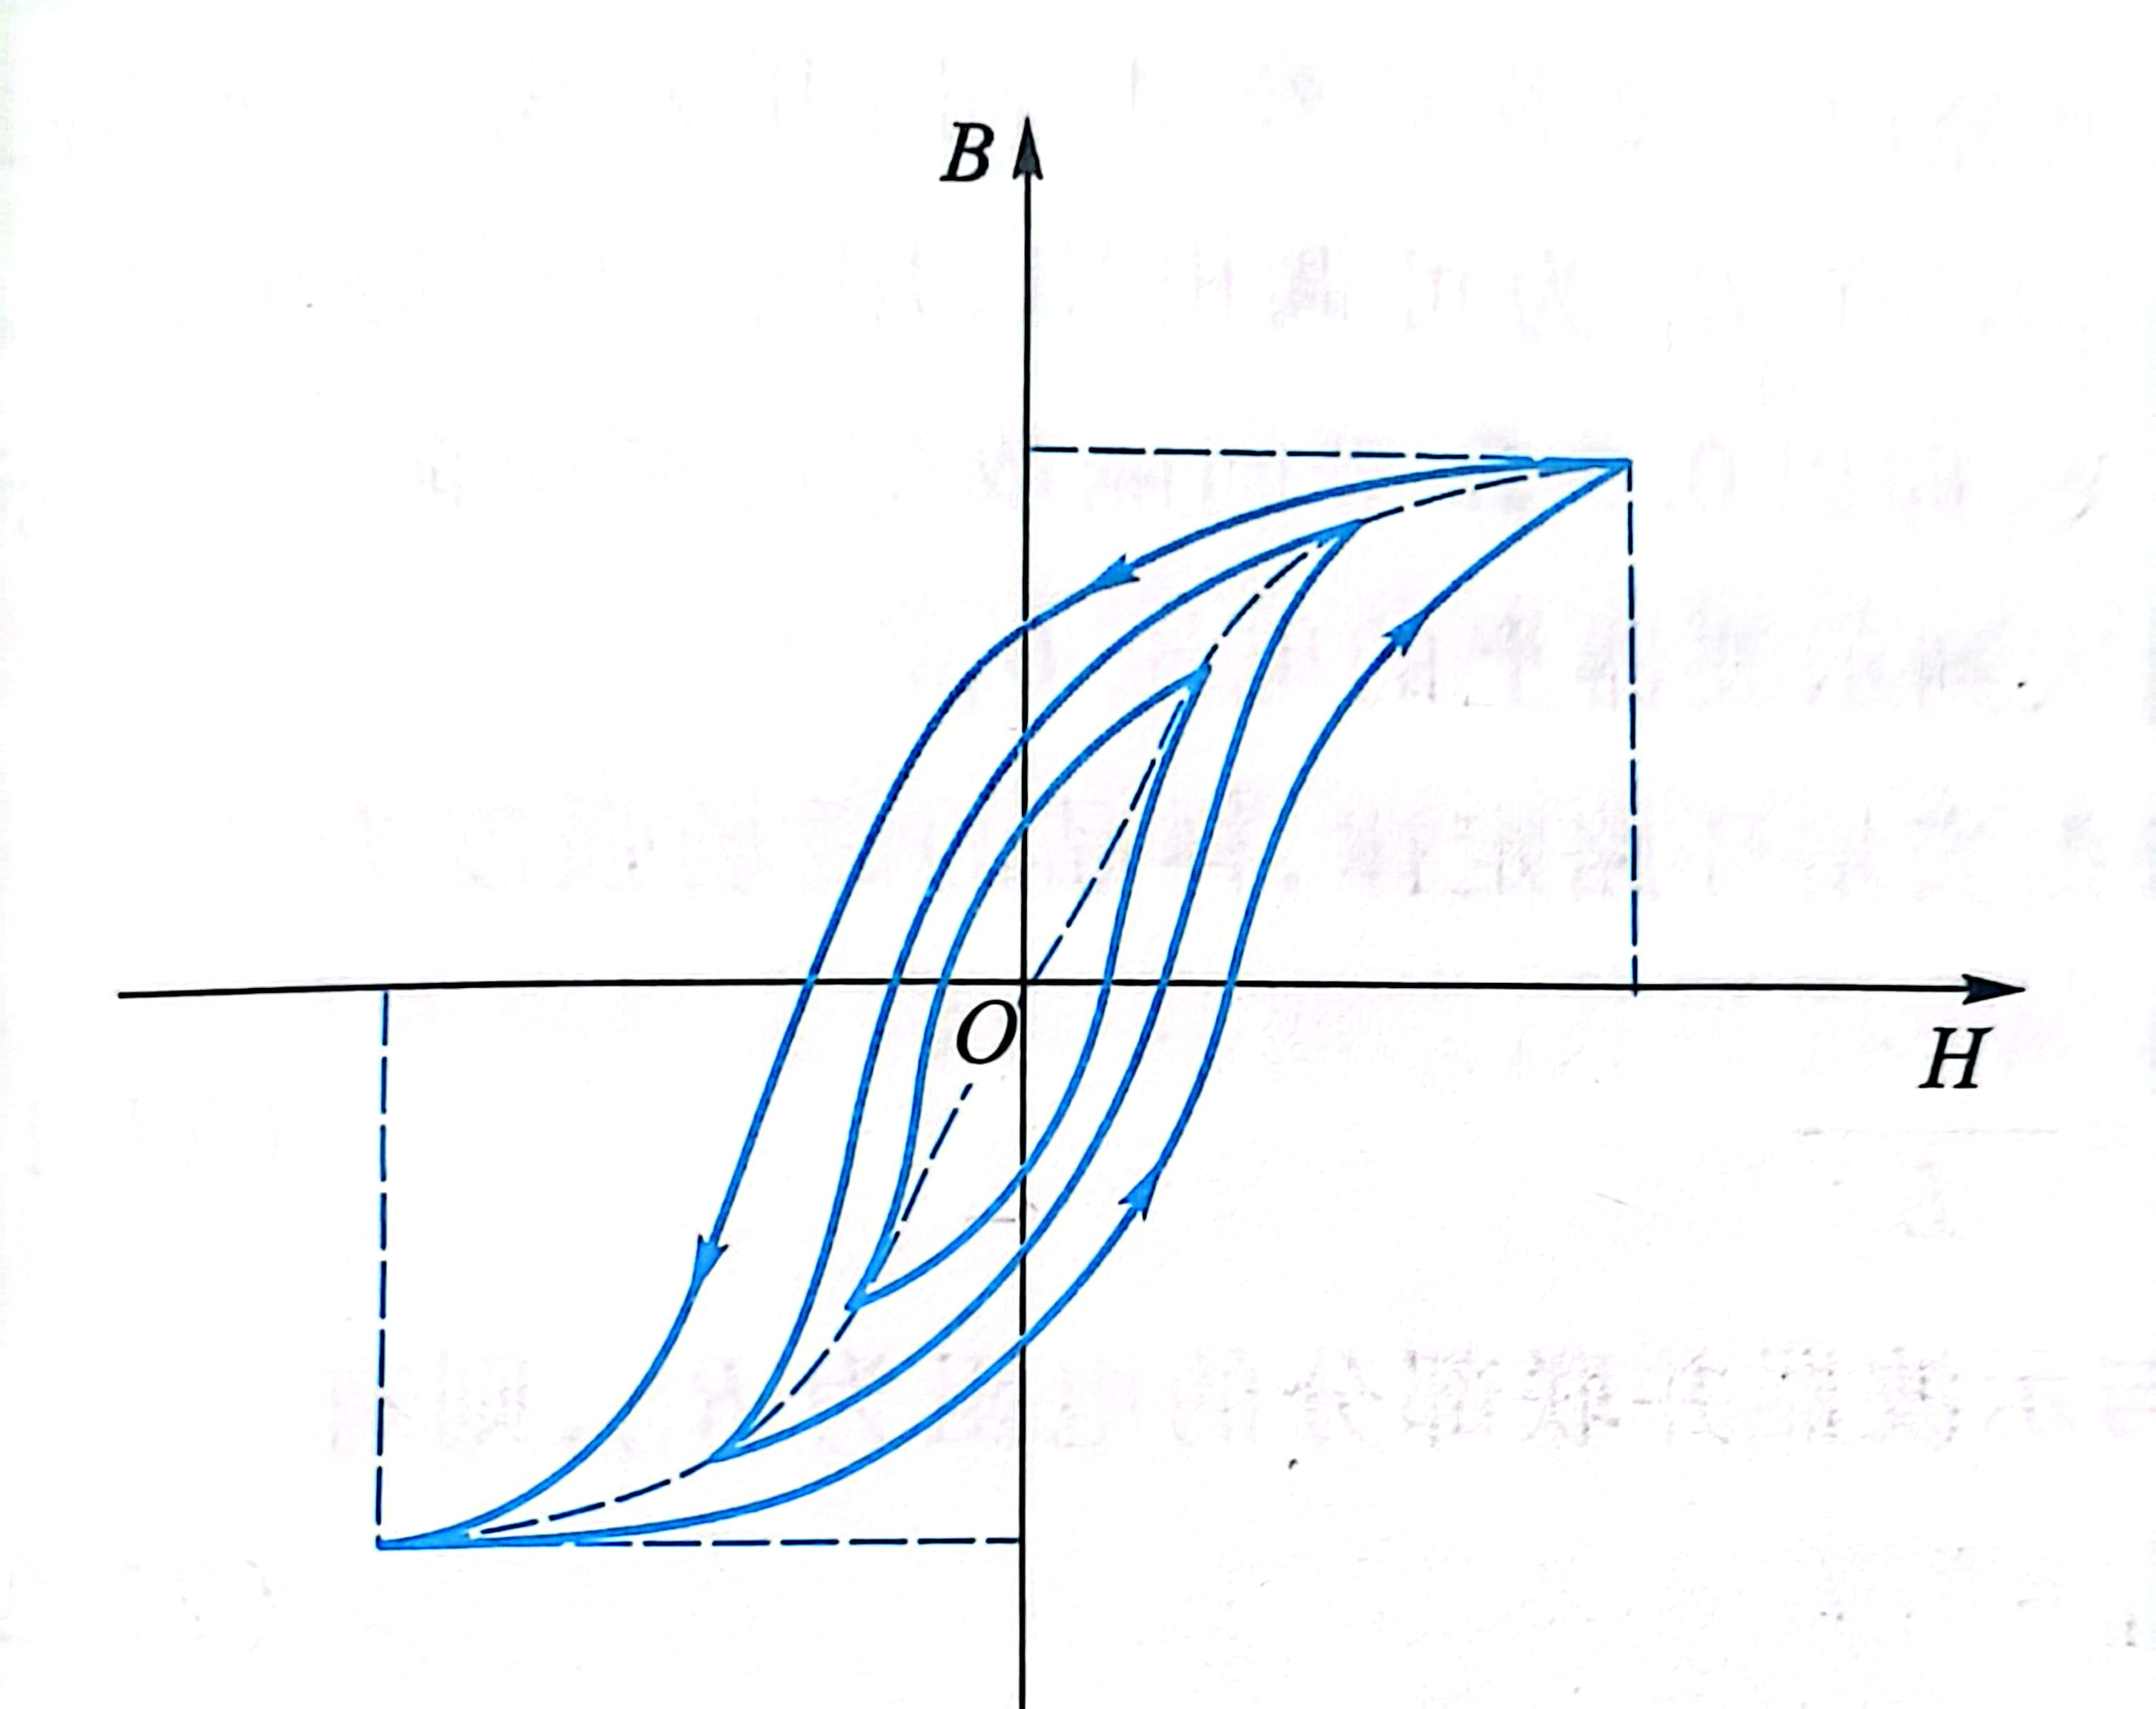
\includegraphics[width=\textwidth,height=0.3\textheight]{tongyicailiaoqvxian.jpg}
      \caption{同一材料的一簇磁滞曲线}
      \label{tongyicailiaoqvxian}
    \end{minipage}
    \begin{minipage}[t]{0.45\textwidth}
      \centering
      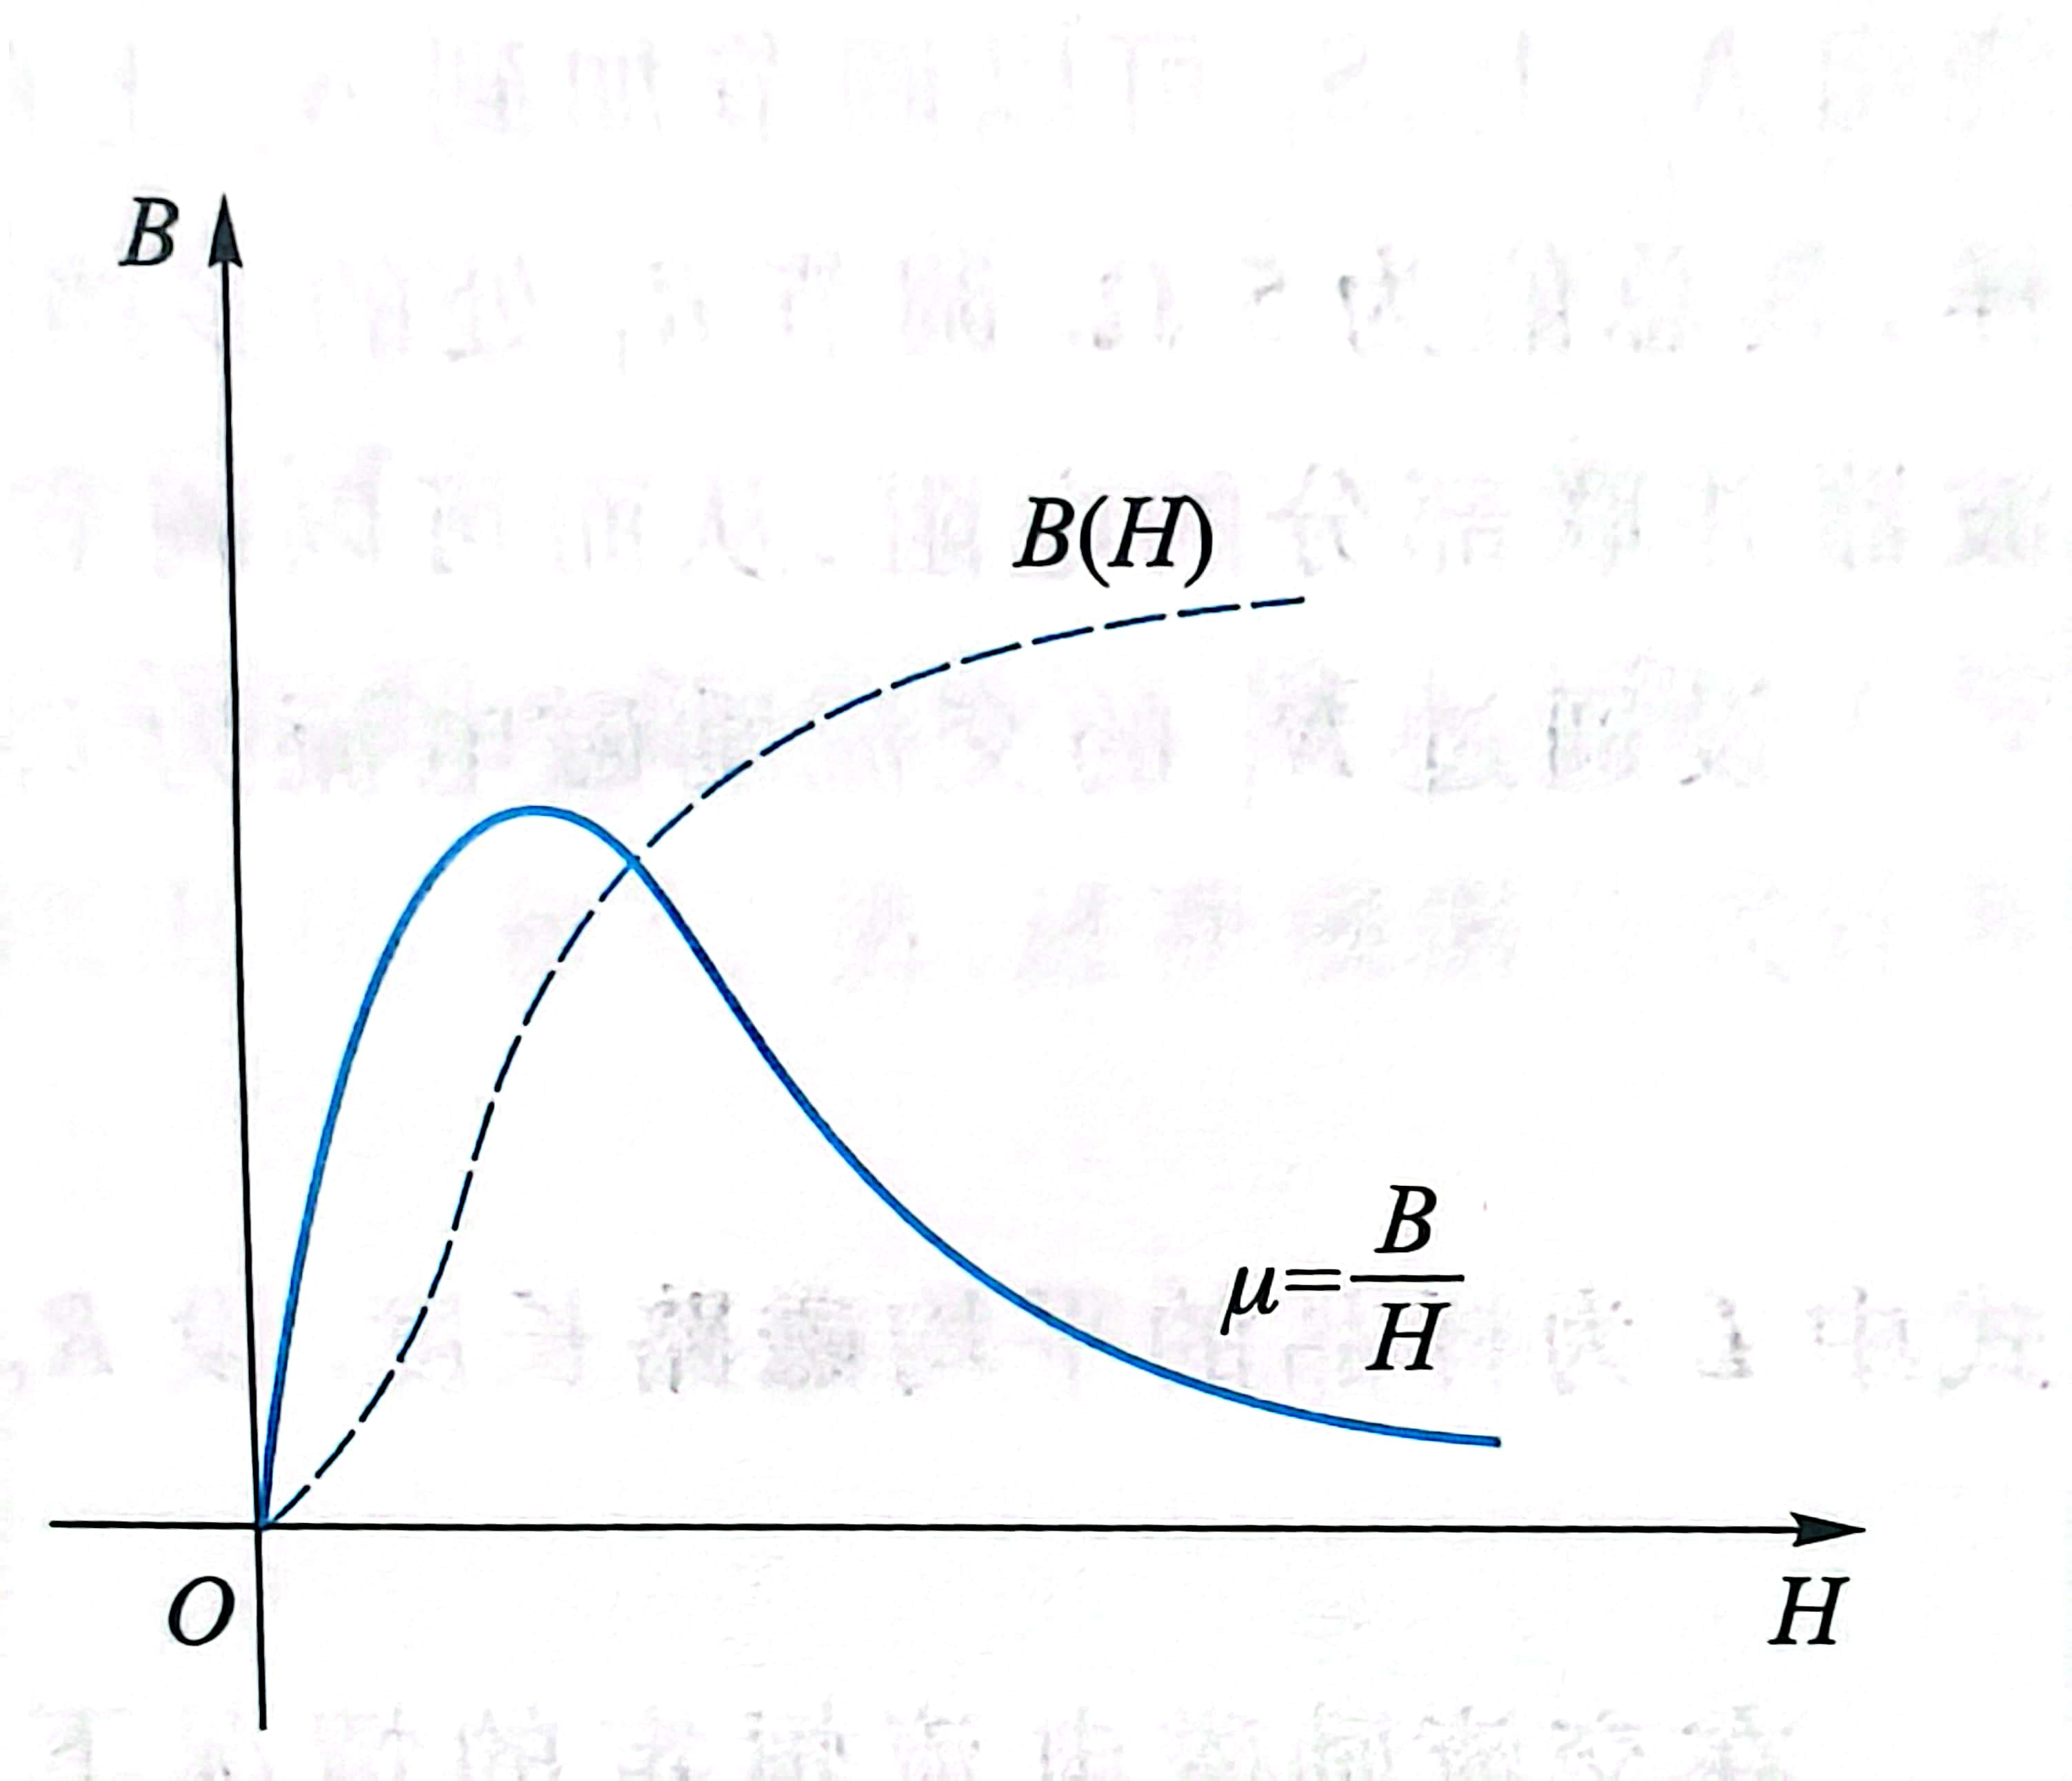
\includegraphics[width=\textwidth,height=0.3\textheight]{muH.jpg}
      \caption{铁磁材料$\mu$和$H$的关系}
      \label{muH}
    \end{minipage}
  \end{figure}

  磁化曲线和磁滞回线是铁磁材料分类和选用的重要依据,图\ref{butongcailiaoqvxian}为常见的两种典型的磁滞回线。
  其中软磁材料磁滞回线狭长,矫顽力、剩磁和磁滞损耗均较小,是制造变压器、电机、和交流磁铁的主要材料;而便磁材料磁滞回线较宽,矫顽力大,剩磁强,可用来制造永磁体。

  \begin{figure}[H]\label{butongcailiaoqvxian}
    \centering
    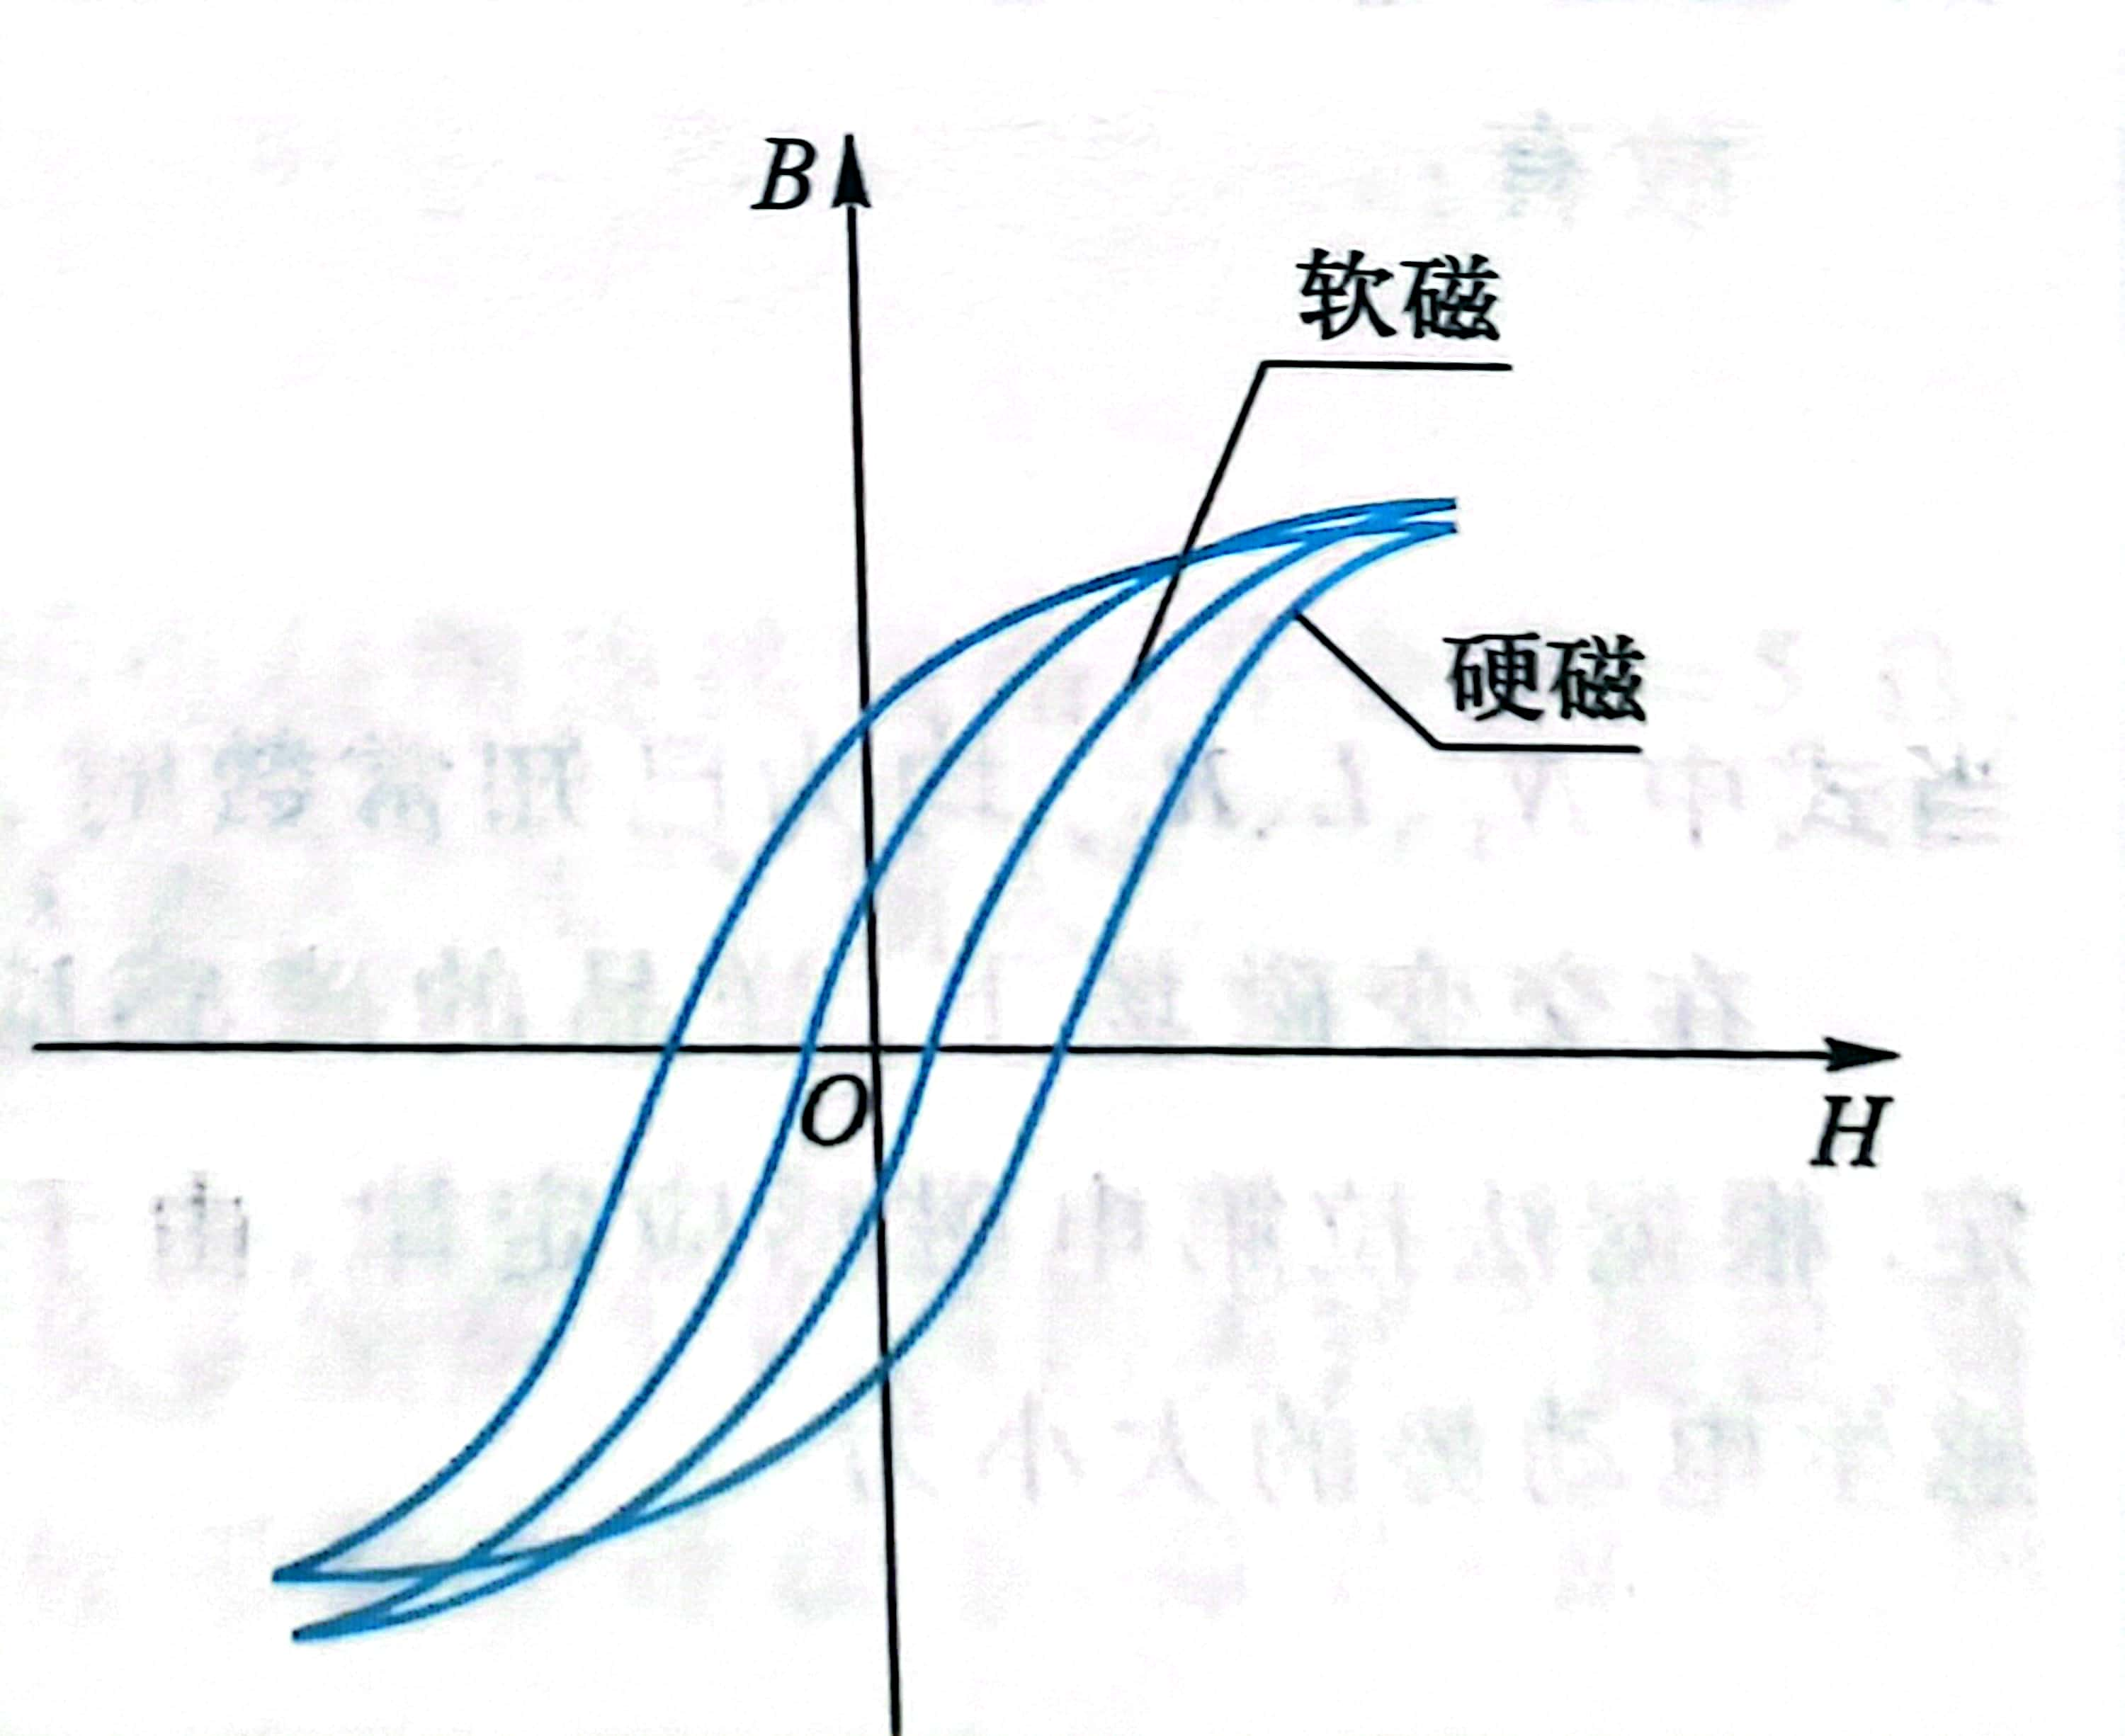
\includegraphics[width=0.5\textwidth,height=0.3\textheight]{butongcailiaoqvxian.jpg}
    \caption{不同材料的磁滞回线}
  \end{figure}


  \subsection{用示波器观察和测量磁滞回线的实验原理和线路}
  在用示波器观察时,示波器工作在XY工作模式,其中x轴输人为磁场强度H,y轴输入为磁感应强度B。观察和测量磁滞回线和基本磁化曲线的线路如图\ref{shiyanyuanliluxian}所示。

  \begin{figure}[H]\label{shiyanyuanliluxian}
    \centering
    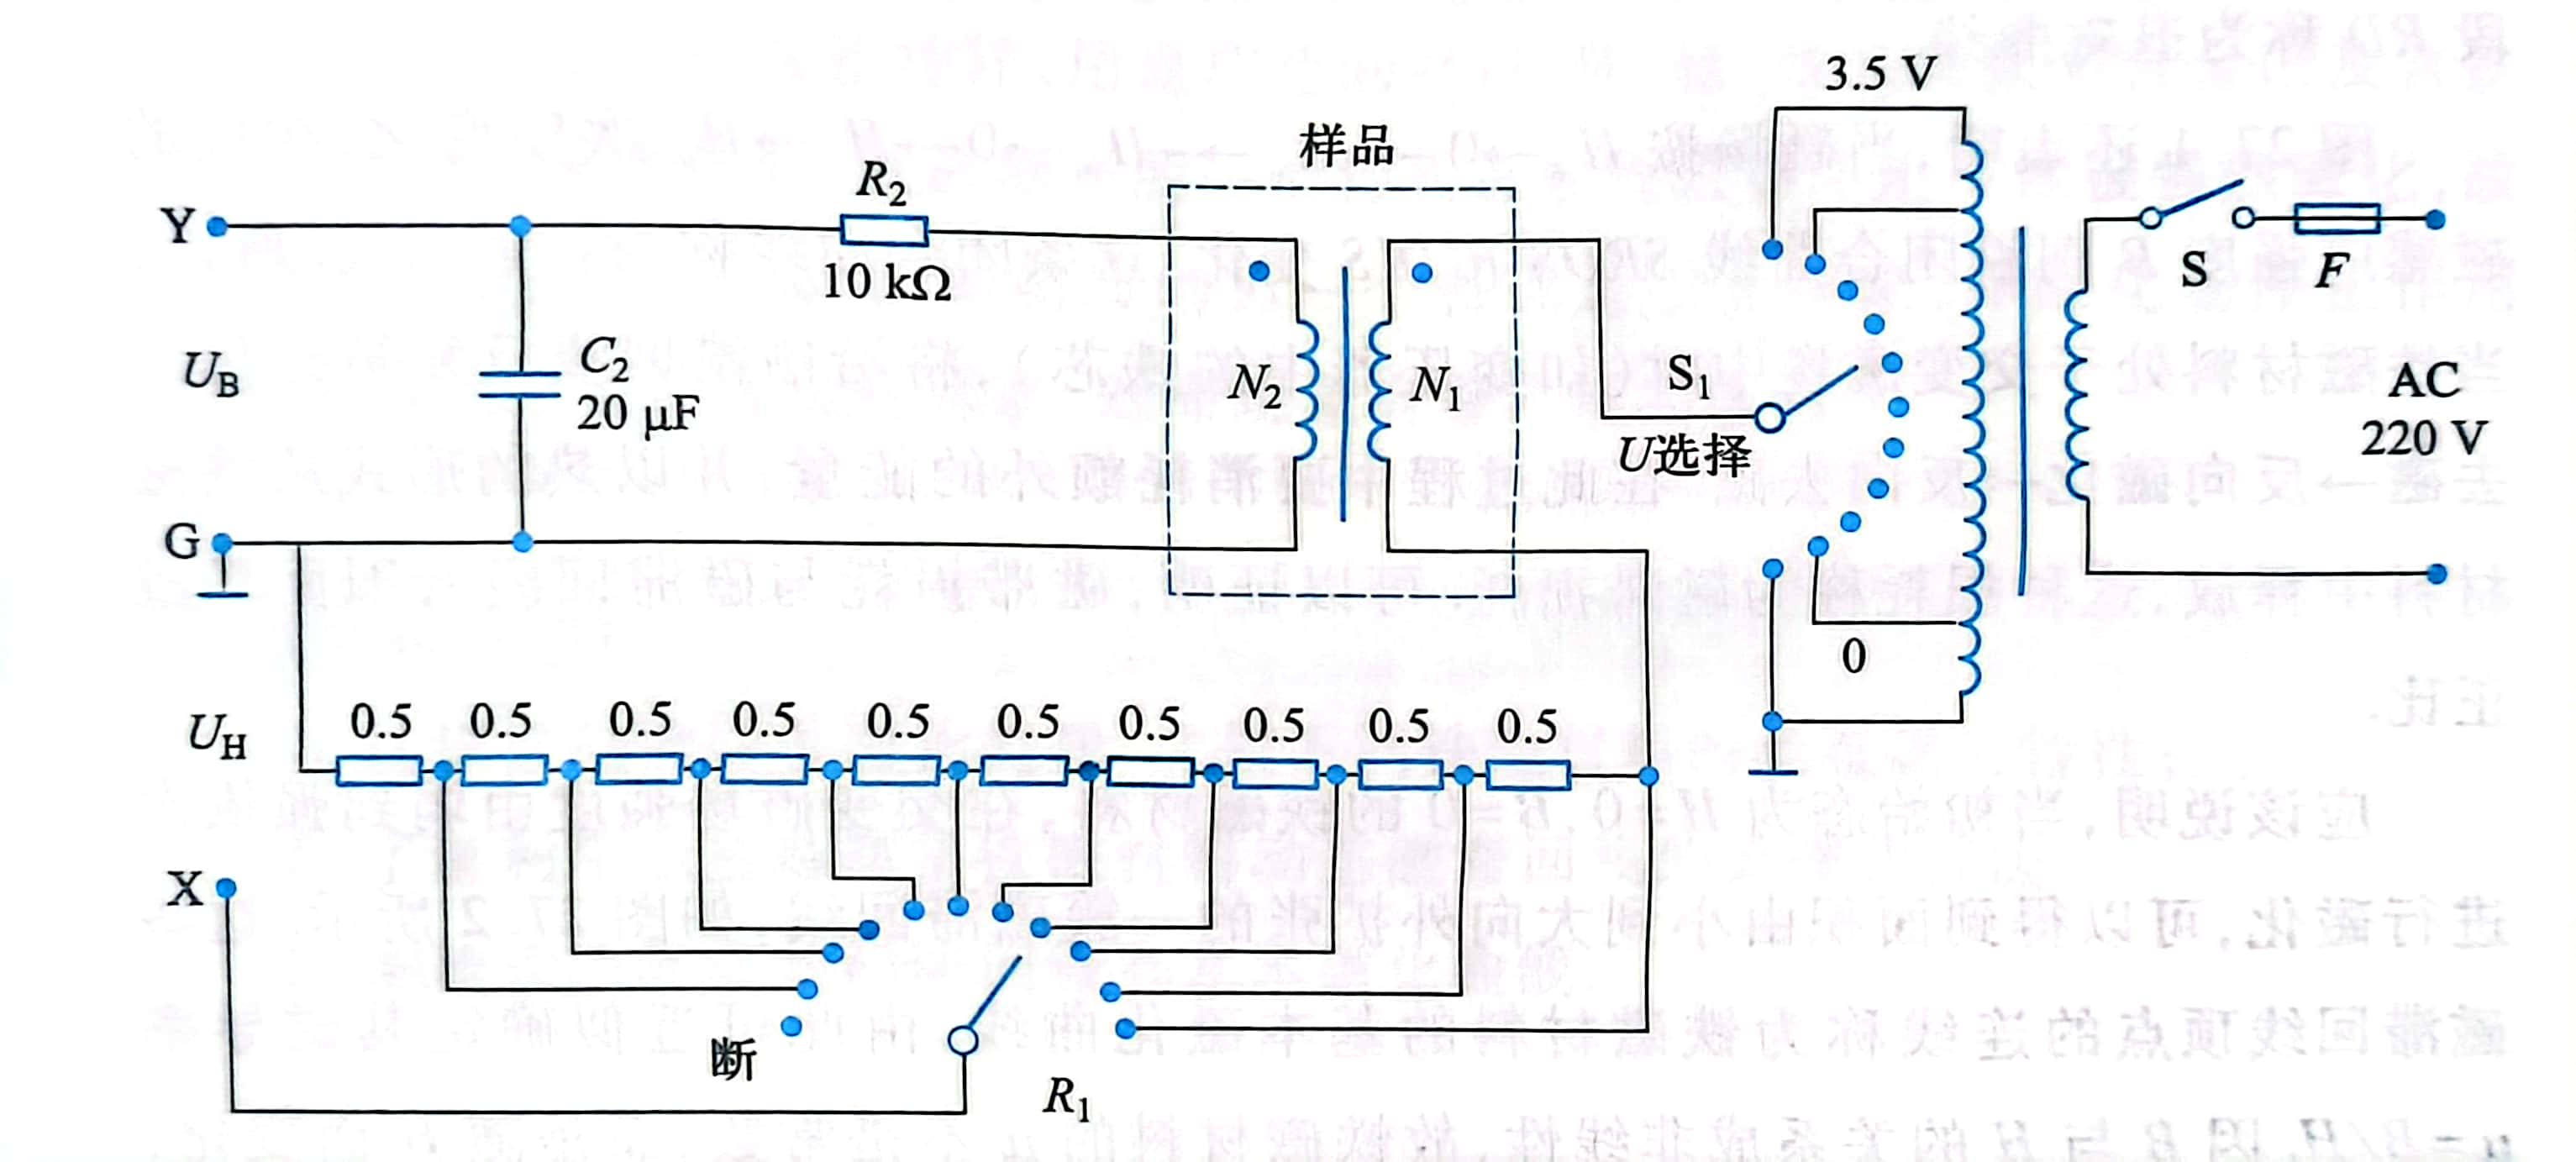
\includegraphics[width=0.9\textwidth,height=0.3\textheight]{shiyanyuanxianlu.jpg}
    \caption{实验原理线路}
  \end{figure}

  在图\ref{shiyanyuanliluxian}中待测样品为EI型砂钢片,被制为闭合的环形,然后均匀绕以励磁线圈$N_{1}$,和测量线圈$N_{2}$。
  220V的交流电经电压变换后经过多挡开关$S_{1}$,加到励磁绕组$N_{1}$上,$S_{1}$可以调节加到$N_{1}$,上的电压值。$R_{1}$为可调电阻,
  用来对励磁电流取样,其总值为5$\Omega$。调节$R_{1}$处的多挡开关,即以$0.5\Omega$等间隔改变可调电阻$R_{1}$与示波器并联部分的电阻,
  从而可以调节输入到示波器上的电压$U_{H}$。

  设通过$N_{1}$的交流励磁电流为i,根据安培环路定律,样品的磁场强度为
  
  \begin{equation}
    H=\frac{N_{1} \cdot i}{L}
  \end{equation}

  式中L为样品的平均磁路长度,设$R_{1}$与示波器并联部分的电阻为$R_{1s}$,则有

  \begin{equation}
    U_{H}=R_{1s}i
  \end{equation}

  在交流励磁电路恒定的情况下,$U_{H}$随可调电阻$R_{1}$的$R_{1s}$部分变大而变大。通过$U_{H}$和$R_{1s}$的值可以得到励磁电流的值。有

  \begin{equation}
    H=\frac{N_{1}}{LR_{1s}} \cdot U_{H}
  \end{equation}

  当式中$N_{i}$、$L$、$R_{1}$均已知的常数时,可由$U_{H}$确定$H$的值。

  在交变磁场下,样品的磁感应强度瞬时值B由测量线圈和$R_{2}C_{2}$电路来确定,
  根据法拉第电磁感应定律,由于样品中磁通量$\Phi$的变化,在测量线圈中产生的感生电动势的大小为
  
  \begin{equation}
    \varepsilon_{2} = N_{2} \frac{d\Phi}{dt}
  \end{equation}

  \begin{equation}
    \Phi = \frac{1}{N_{2}} \int \varepsilon_{2}dt 
  \end{equation}

  \begin{equation}
    B=\frac{\varepsilon}{S}=\frac{1}{N_{2}S} \int \varepsilon dt
  \end{equation}

  式中S为样品的截面积。

  如果忽略自感电动势和电路损耗,则回路方程为
  
  \begin{equation}
    \varepsilon_{2} = i_{2} R_{2} + U_{B}
  \end{equation}

  式中$i_{2}$为感生电流,$U_{B}$为积分电容$C_{2}$两端电压,设在$\Delta t$时间内$i_{2}$向电容$C_{2}$
  充电电荷量为Q,则有

  \begin{equation}
    U_{B}=\frac{Q}{C_{2}}
  \end{equation}

  \begin{equation}
    \varepsilon_{2} = i_{2}R_{2} + \frac{Q}{C_{2}}
  \end{equation}

  如果选取足够大的$R_{2}$和$C_{2}$,使$i_{2}R_{2}>>\frac{Q}{c_{2}}$

  \begin{equation}
    \varepsilon_{2}=i_{2}R_{2}=\frac{dQ}{dt}R_{2}=C_{2}\frac{dU_{B}}{dt}R_{2}
  \end{equation}

  上式中可由$U_{B}$确定$B$,则有

  \begin{equation}
    B=\frac{C_{2}R_{2}}{N_{2}S} U_{B}
  \end{equation}

  综上所述,只要将$U_{H}$和$U_{B}$分别加到示波器的“X输入”和“Y输人”便可观察样品的B-H曲线,并可用示波器测出$U_{H}$和$U_{B}$值,进而根据公式计算出B和H。

\section{实验装置器材介绍}
磁滞回线实验仪、示波器

\section{实验内容及实验步骤}
  \subsection{电路连接}
  选择硅钢片材料(蓝色)磁芯,按电路图连接线路,并令$R_{1}=5\Omega$,“U选择”置于0位。$U_{H}$和$U_{B}$,分别接示波器的“X输入”和“Y输入”。

  \subsection{样品退磁}
  开启实验仪电源,转动“U选择”旋钮,令U从0增至3V,然后再转动旋钮,将U从最大值降为0,从而消除剩磁,确保样品处于磁中性状态,即B=H=0,如图\ref{tuicishiyi}所示.

  \begin{figure}[H]
    \begin{minipage}[t]{0.45\textwidth}
      \centering
      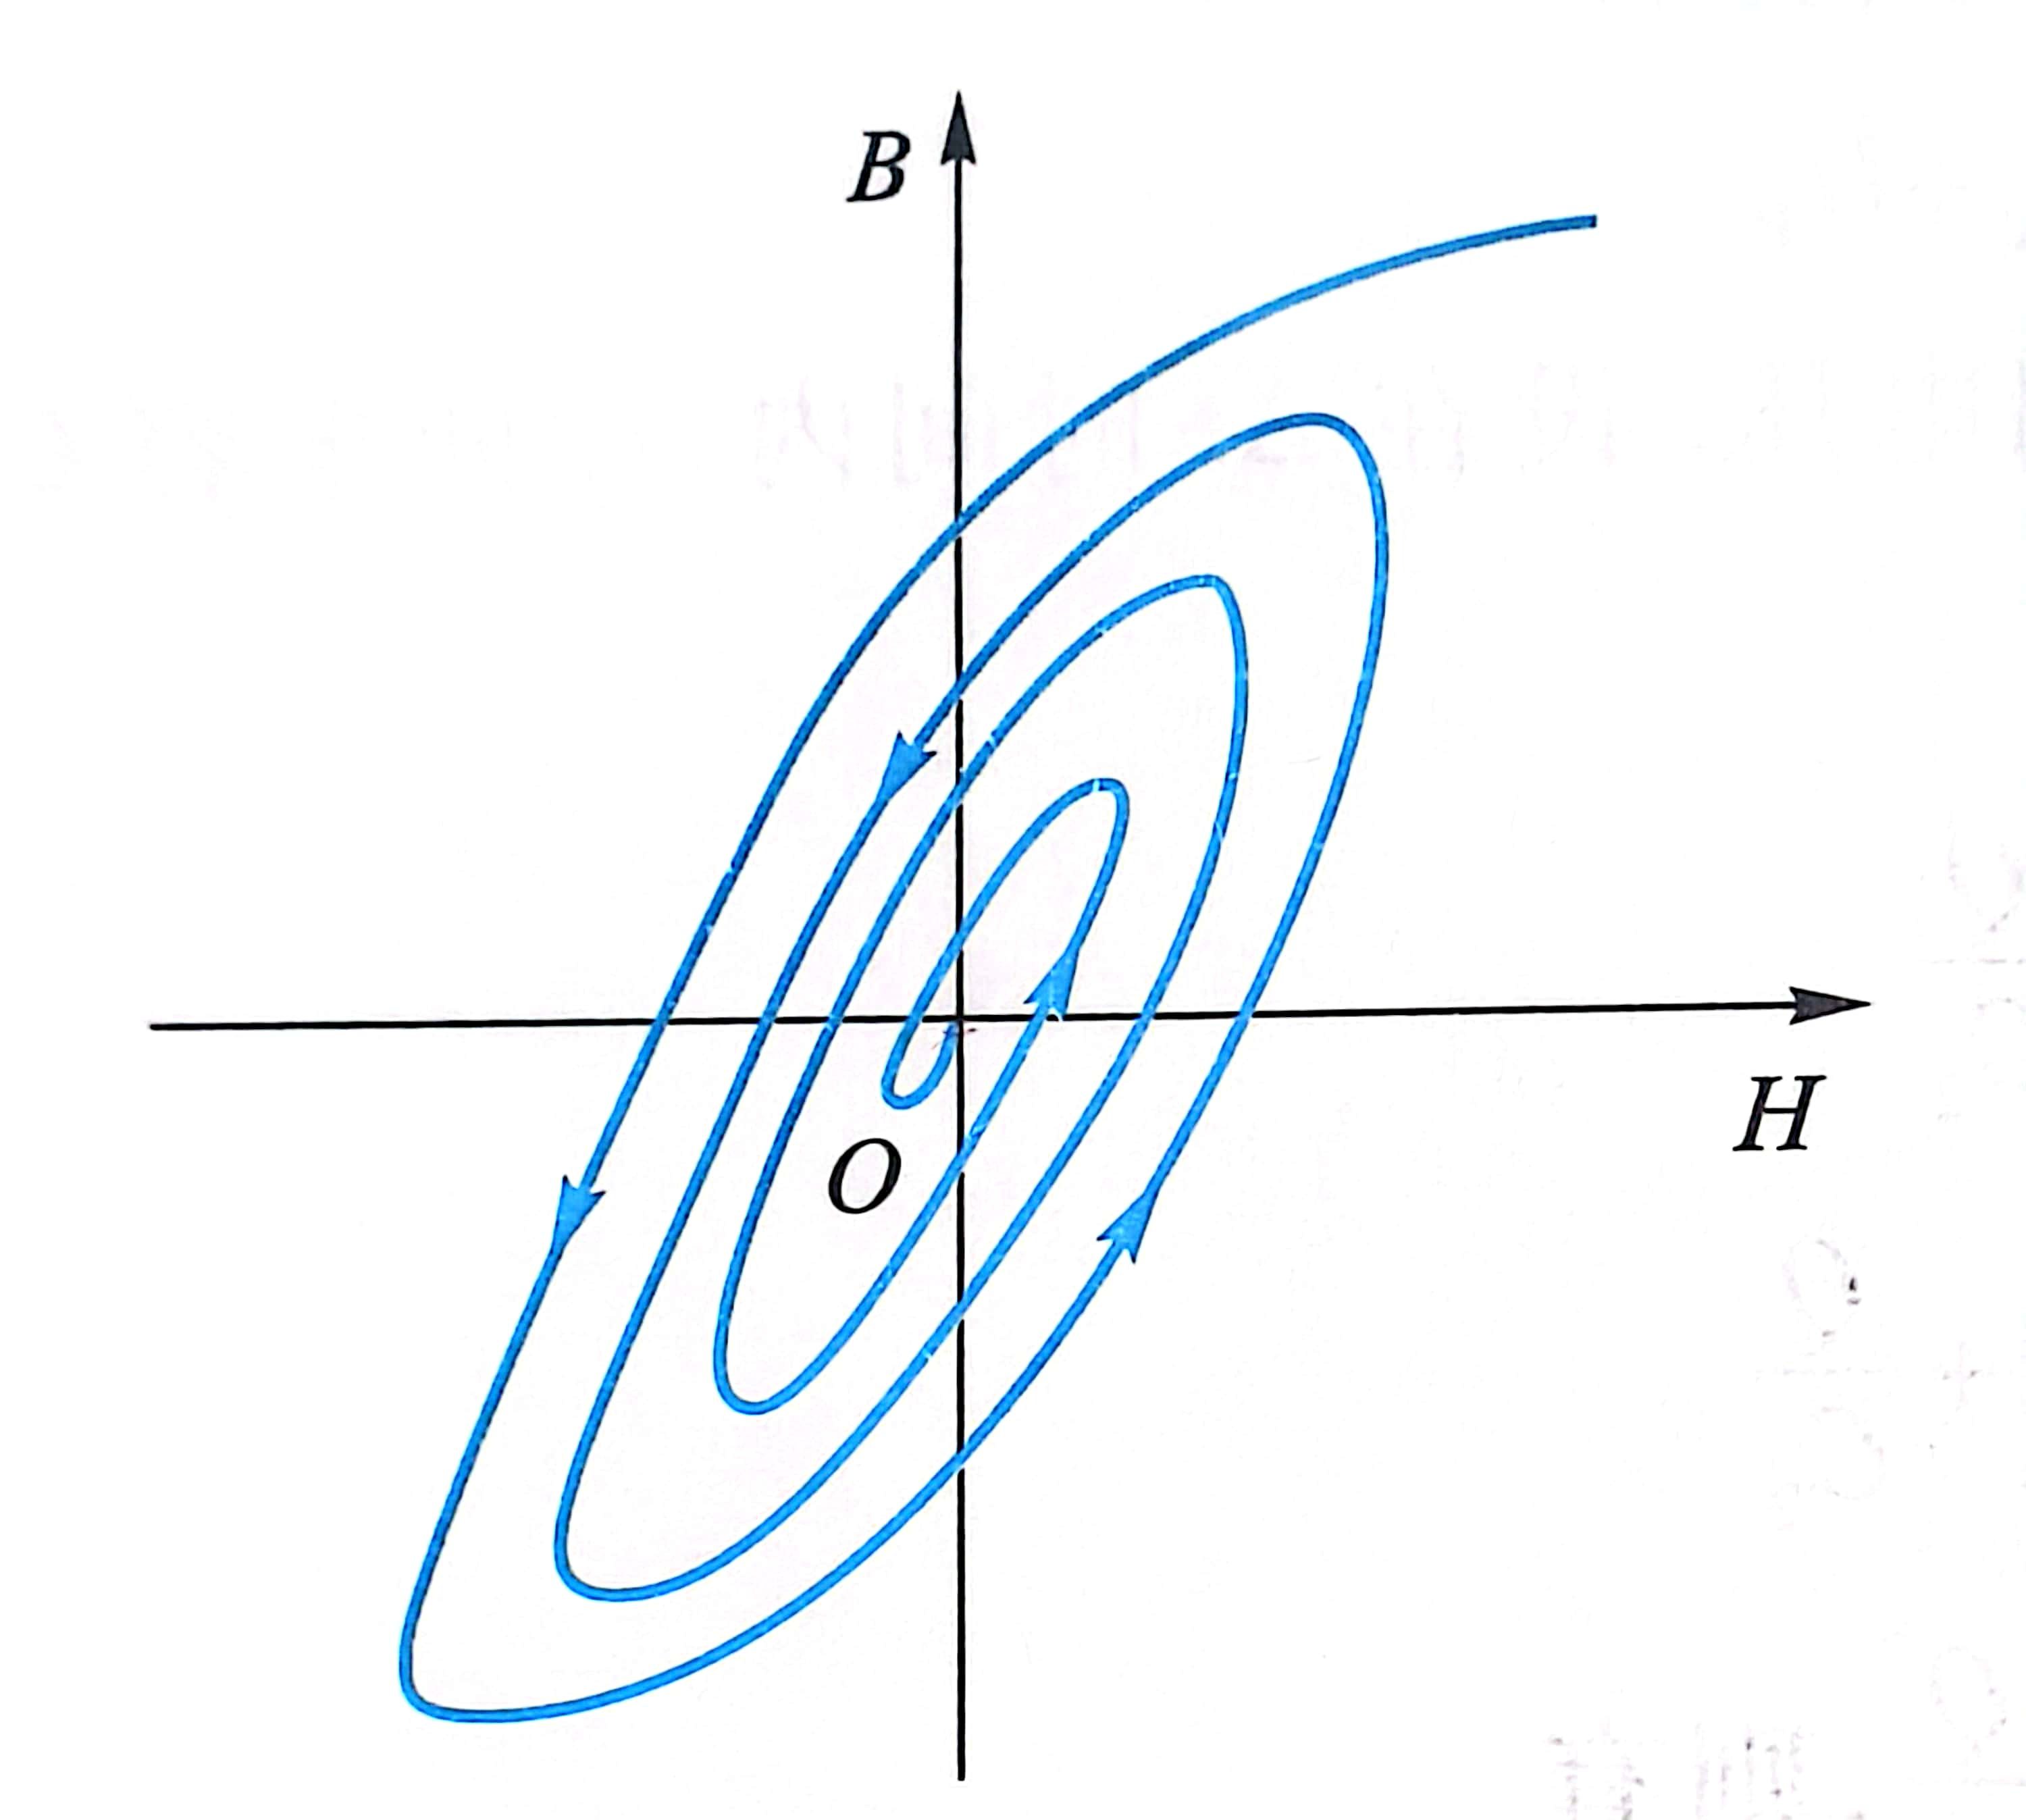
\includegraphics[width=\textwidth,height=0.3\textheight]{tuicishiyi.jpg}
      \caption{退磁示意图}
      \label{tuicishiyi}
    \end{minipage}
    \begin{minipage}[t]{0.45\textwidth}
      \centering
      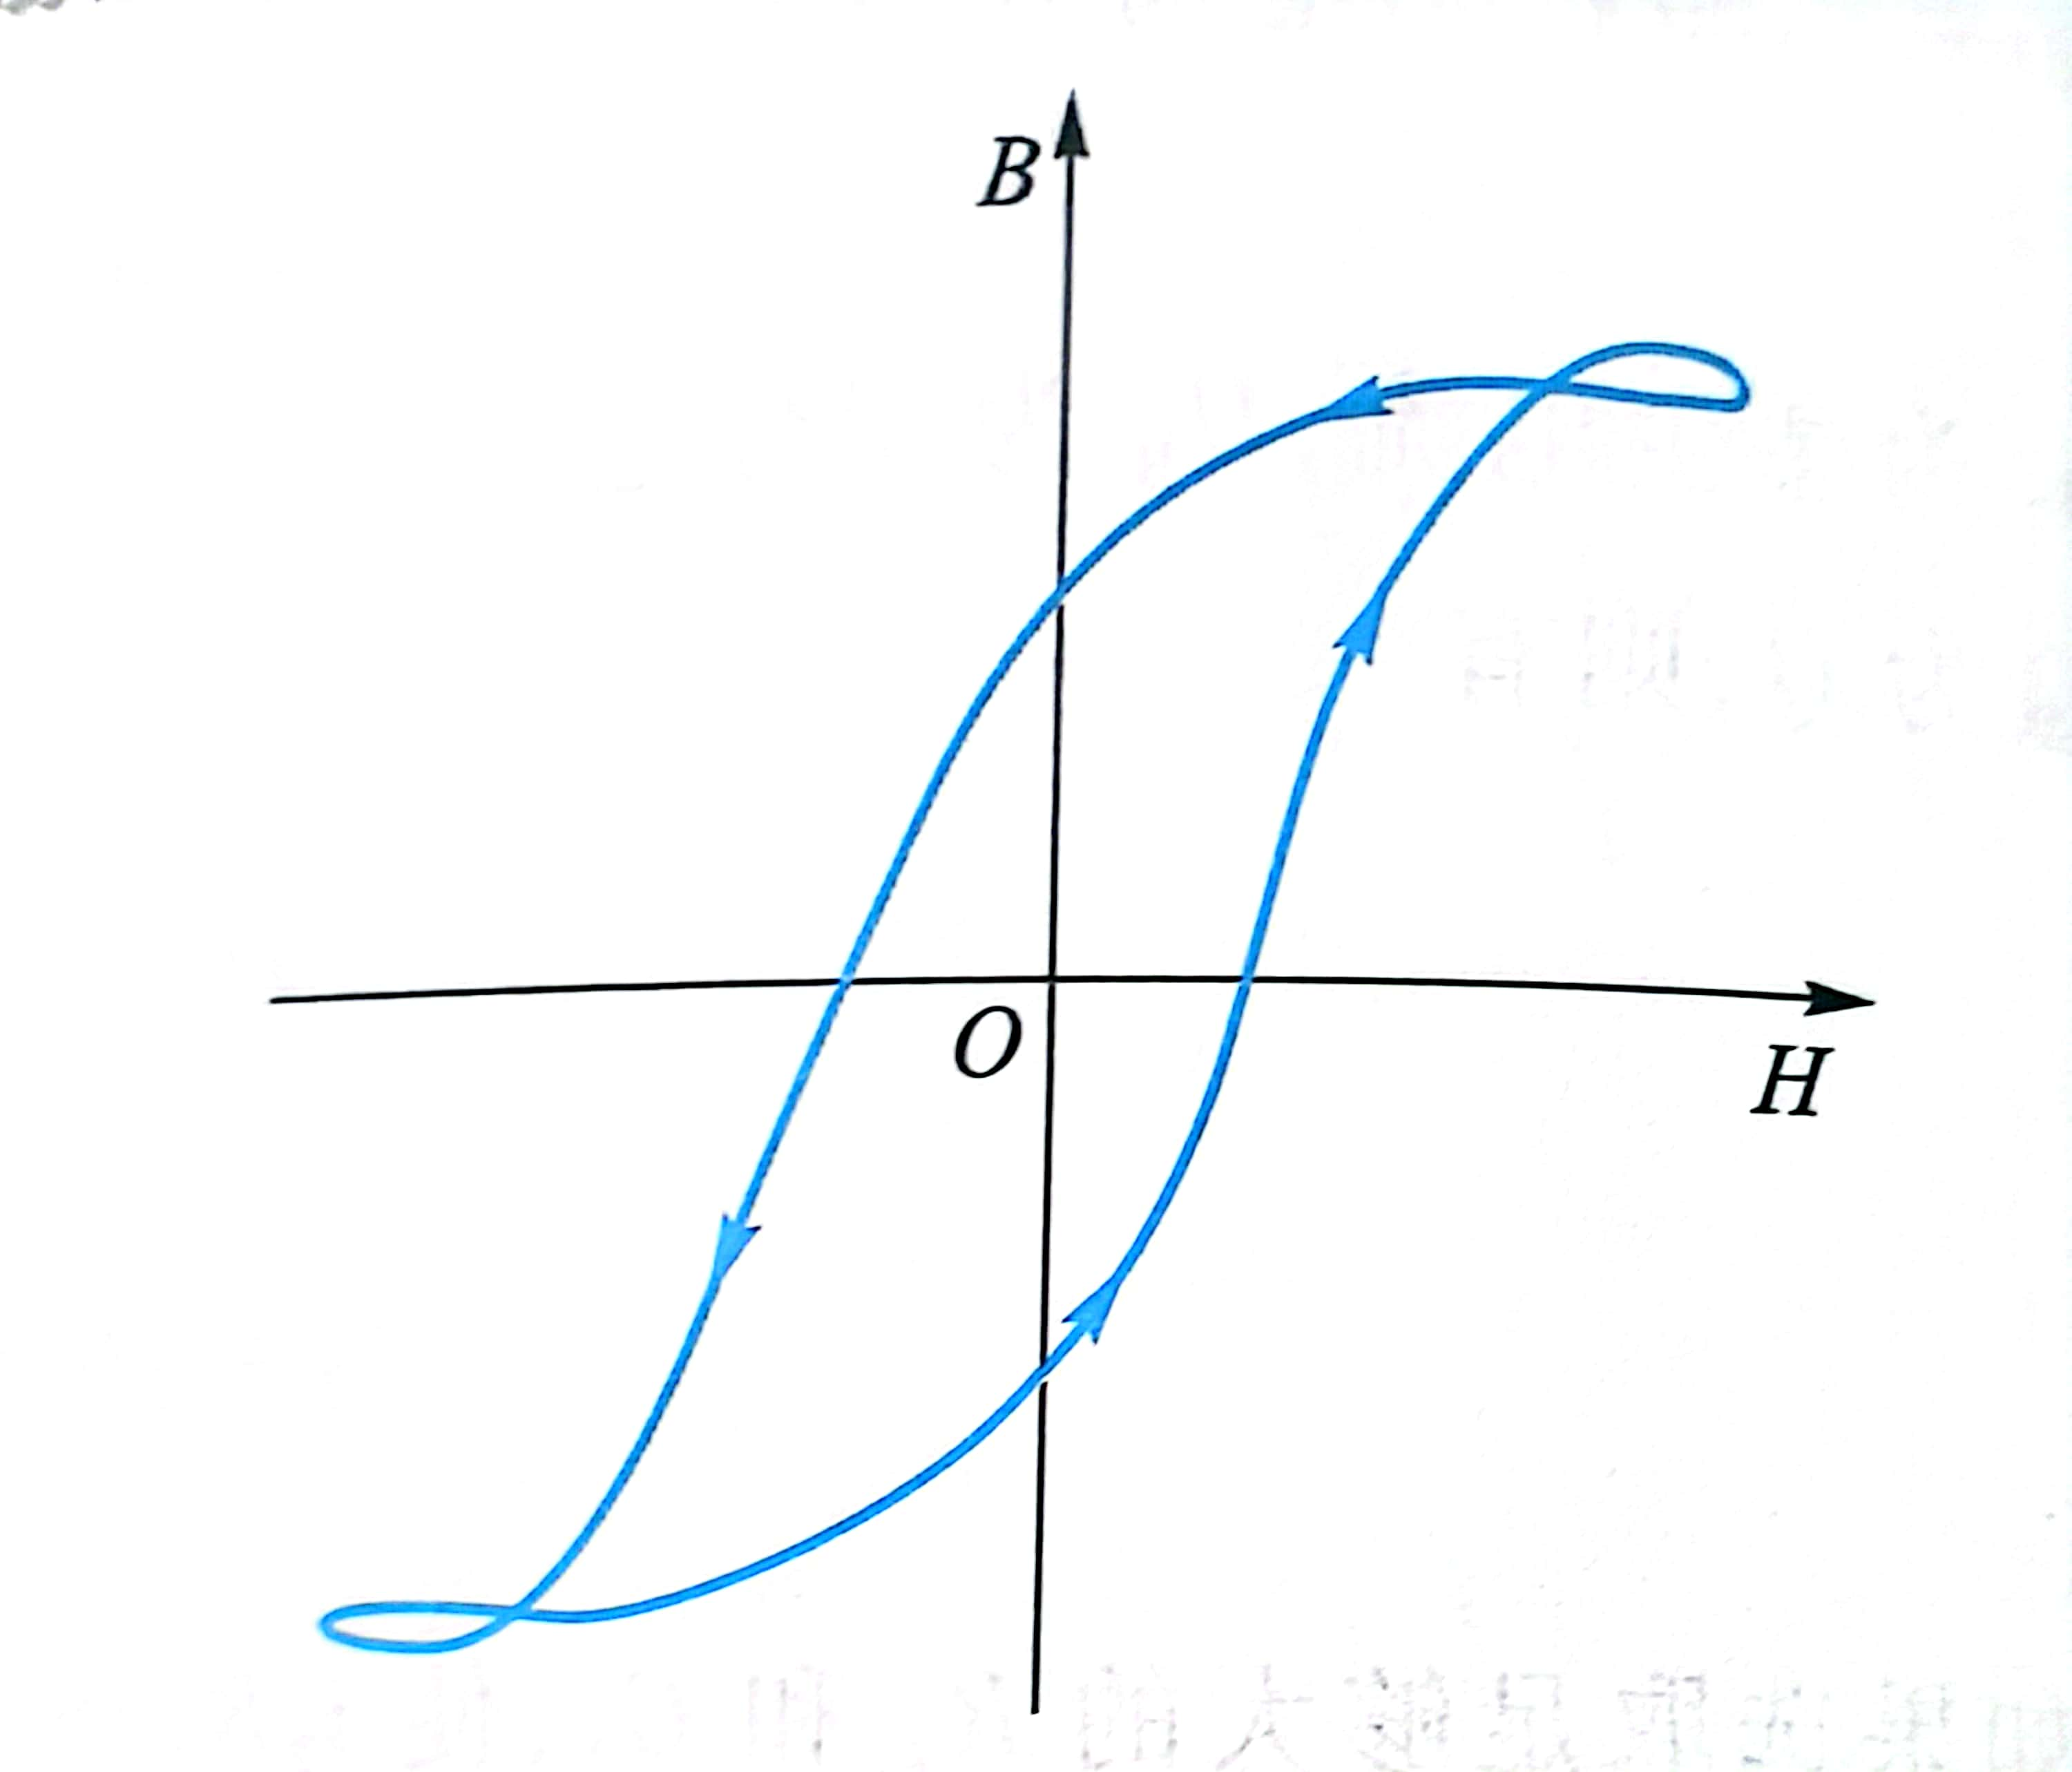
\includegraphics[width=\textwidth,height=0.3\textheight]{jibianxianxiang.jpg}
      \caption{调节不当引起的畸变现象}
      \label{jibianxianxiang}
    \end{minipage}
  \end{figure}

  \subsection{观察退磁回线}
  令U=3.0V,开启示波器电源,并分别调节示波器X和Y轴的灵敏度,使显示屏上出现图形大小合适的磁滞回线,
  若图形顶部出现编织状的小环,如图\ref{jibianxianxiang}所示,这时应该检查示波器的通道输入方式,
  一般应选择“DC”,或者X通道“AC”,Y通道“DC”,并适当选择$R_{1}$值,或降低励磁电压U予以消除。

  \subsection{观察基本磁化曲线}
  按步骤2对样品进行退磁,从U=0开始,
  逐挡提高励磁电压,将在显示屏上得到面积由小到大一个套一个的一簇磁滞回线,
  记录下这些磁滞回线顶点的B和H的值,并将B和H的值作图连线就是样品的基本磁化曲线。

  \subsection{已知条件}
  调节U=3.0 V,$R_{1}=5\Omega$,测定样品的一组$U_{B}$、$U_{H}$值,并根据已知条件:L= 75 mm,S=120 $mm^{2}$,
  $C_{2}=20\mu F$,$R_{2}=10k\Omega$,N=60匝,计算出相应的B和H的值。


  \subsection{$W_{BH}$}
  根据得到的B和H的值作B-H曲线,根据曲线求得$B_{m}B_{r}H_{e}$等参数,并估算曲线的面积来求得$W_{BH}$。

  \subsection{$\mu - H$曲线}
  依次测定U=0.5、1.0、\dots、3.5V十组$U_{H}U_{B}$,计算得出相应的$H_{m}H_{m}\mu$,作出$\mu - H$曲线。


  \subsection{不同曲线观察}
  改变$R_{1}$,观察不同的磁化曲线。

  \subsection{二次测量}
  更换样品为另一个磁芯($N_{1}=90$匝),重复上述步骤,并对比两种材料的测量结果。
\newpage

\section{实验原始数据}
\begin{figure}[H]
  \centering
  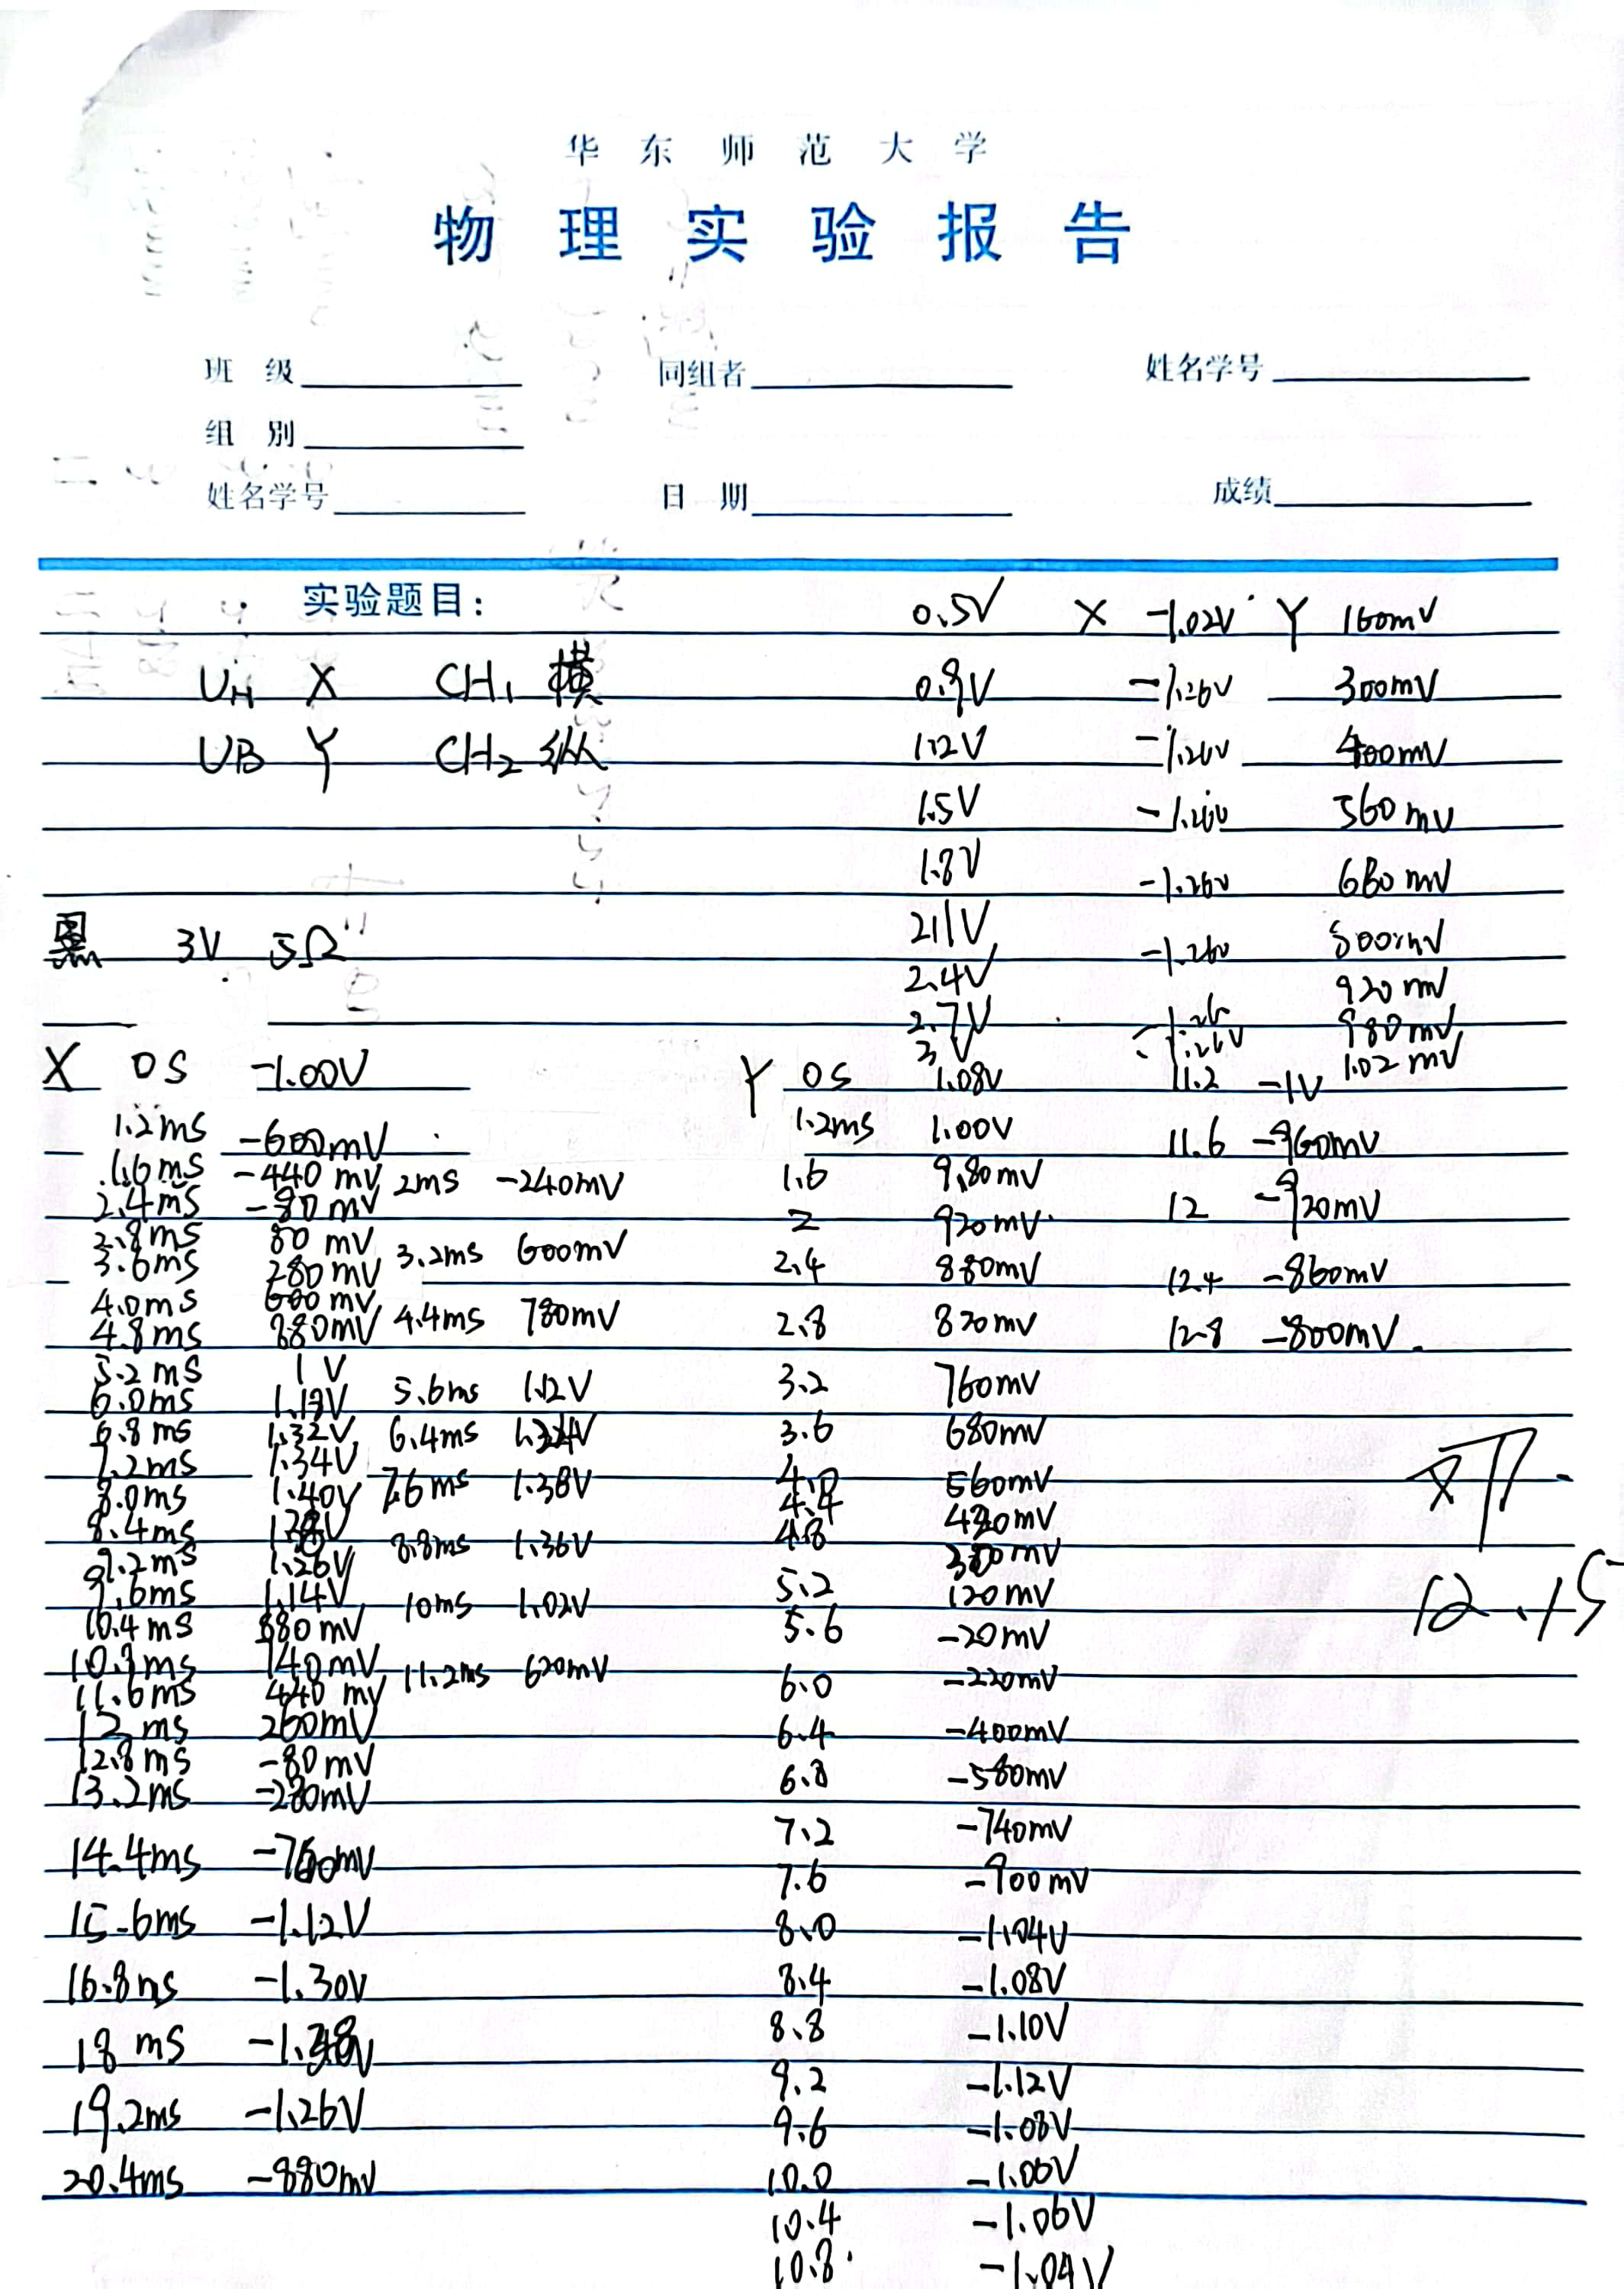
\includegraphics[width=0.9\textwidth,height=0.8\textheight]{yuanshishujv1.jpg}
  \caption{实验原始数据1}
\end{figure}
\newpage

\begin{figure}[H]
  \centering
  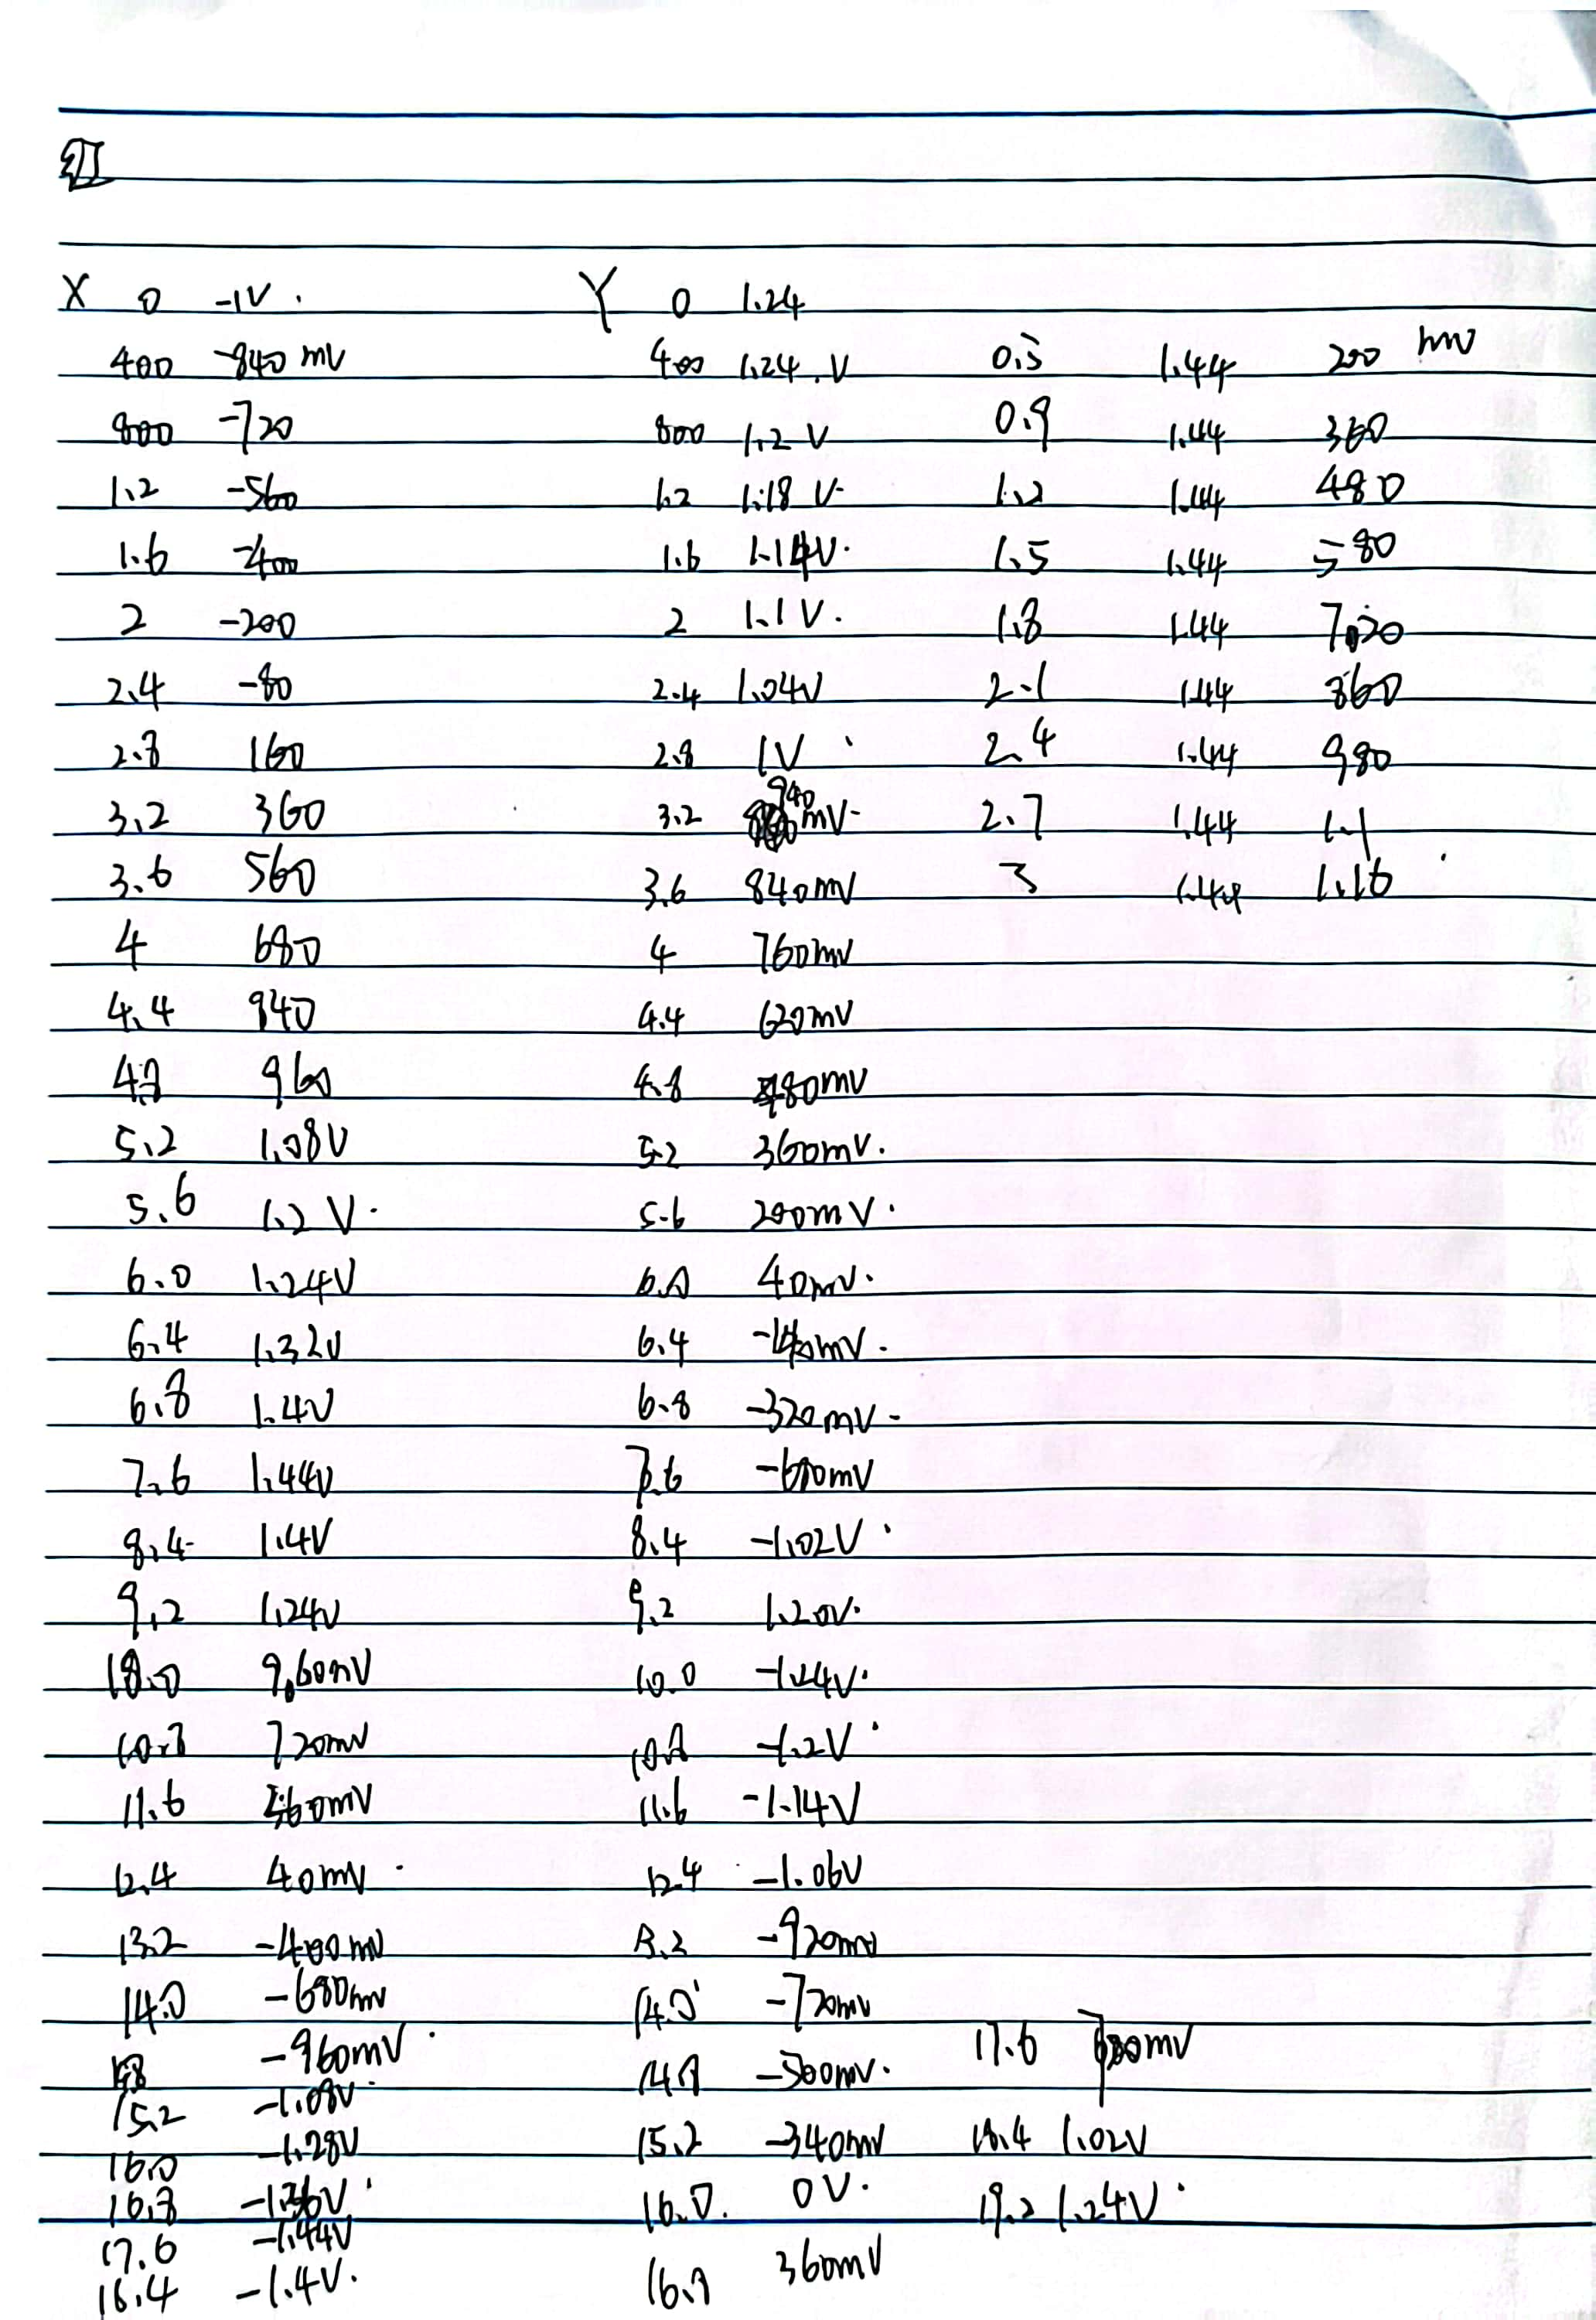
\includegraphics[width=0.9\textwidth,height=0.8\textheight]{yuanshishujv2.jpg}
  \caption{实验原始数据2}
\end{figure}
\newpage







\section{实验数据处理}

\section{思考题}
  \subsection{思考题一}

  \subsection{思考题二}

\section{实验中个人的思考与感想}
  \subsection{对于实验个人观点}

  \subsection{实验中的总结}

\end{document}
